% A LaTeX template for MSc Thesis submissions to 
% Politecnico di Milano (PoliMi) - School of Industrial and Information Engineering
%
% S. Bonetti, A. Gruttadauria, G. Mescolini, A. Zingaro
% e-mail: template-tesi-ingind@polimi.it
%
% Last Revision: October 2021
%
% Copyright 2021 Politecnico di Milano, Italy. NC-BY

\documentclass{Configuration_Files/PoliMi3i_thesis}

%------------------------------------------------------------------------------
%	REQUIRED PACKAGES AND  CONFIGURATIONS
%------------------------------------------------------------------------------

% CONFIGURATIONS
\usepackage{parskip} % For paragraph layout
\usepackage{setspace} % For using single or double spacing
\usepackage{emptypage} % To insert empty pages
\usepackage{multicol} % To write in multiple columns (executive summary)
\usepackage{enumerate}
\setlength\columnsep{15pt} % Column separation in executive summary
\setlength\parindent{0pt} % Indentation
\raggedbottom  

% PACKAGES FOR TITLES
\usepackage{titlesec}
% \titlespacing{\section}{left spacing}{before spacing}{after spacing}
\titlespacing{\section}{0pt}{3.3ex}{2ex}
\titlespacing{\subsection}{0pt}{3.3ex}{1.65ex}
\titlespacing{\subsubsection}{0pt}{3.3ex}{1ex}
\usepackage{color}

% PACKAGES FOR LANGUAGE AND FONT
\usepackage[english]{babel} % The document is in English  
\usepackage[utf8]{inputenc} % UTF8 encoding
\usepackage[T1]{fontenc} % Font encoding
\usepackage[11pt]{moresize} % Big fonts

% PACKAGES FOR IMAGES
\usepackage{graphicx}
\usepackage{transparent} % Enables transparent images
\usepackage{eso-pic} % For the background picture on the title page
%\usepackage{subfig} % Numbered and caption subfigures using \subfloat.
\usepackage{tikz} % A package for high-quality hand-made figures.
\usepackage{forest}
\usepackage[T1]{fontenc}
\usetikzlibrary{shapes.geometric, arrows.meta, positioning}
\usepackage{dirtree}

\graphicspath{{./Images/}} % Directory of the images
\usepackage{caption} % Coloured captions
\usepackage{xcolor} % Coloured captions
\usepackage{amsthm,thmtools,xcolor} % Coloured "Theorem"
\usepackage{float}
\usepackage{physics}
\usepackage{siunitx}
% STANDARD MATH PACKAGES
\usepackage{amsmath}
\usepackage{amsthm}
\usepackage{amssymb}
\usepackage{amsfonts}
\usepackage{bm}
\usepackage[overload]{empheq} % For braced-style systems of equations.
\usepackage{fix-cm} % To override original LaTeX restrictions on sizes

% PACKAGES FOR TABLES
\usepackage{tabularx}
\usepackage{longtable} % Tables that can span several pages
\usepackage{colortbl}
\usepackage{multirow}
\usepackage{booktabs}

% PACKAGES FOR ALGORITHMS (PSEUDO-CODE)
\usepackage{algorithm}
\usepackage{algorithmic}

% PACKAGES FOR REFERENCES & BIBLIOGRAPHY
\usepackage[colorlinks=true,linkcolor=black,anchorcolor=black,citecolor=black,filecolor=black,menucolor=black,runcolor=black,urlcolor=black]{hyperref} % Adds clickable links at references
\usepackage{cleveref}
\usepackage[square, numbers, sort&compress]{natbib} % Square brackets, citing references with numbers, citations sorted by appearance in the text and compressed
\bibliographystyle{abbrvnat} % You may use a different style adapted to your field

% OTHER PACKAGES
\usepackage{pdfpages} % To include a pdf file
\usepackage{afterpage}
\usepackage{lipsum} % DUMMY PACKAGE
\usepackage{fancyhdr} % For the headers
\usepackage{subcaption}
\fancyhf{}

% Input of configuration file. Do not change config.tex file unless you really know what you are doing. 
\input{Configuration_Files/config}

%----------------------------------------------------------------------------
%	NEW COMMANDS DEFINED
%----------------------------------------------------------------------------

% EXAMPLES OF NEW COMMANDS
\newcommand{\R}{\mathbf{R}}
\newcommand{\C}{\mathbf{C}}
\newcommand{\pauli}{\boldsymbol{\sigma}}
\newcommand{\bea}{\begin{eqnarray}} % Shortcut for equation arrays
\newcommand{\eea}{\end{eqnarray}}
\newcommand{\e}[1]{\times 10^{#1}}  % Powers of 10 notation
\newcommand{\bbcs}{\bra{\text{BCS}}}
\newcommand{\bcs}{\ket{\text{BCS}}}
\newcommand{\explaindelta}{$\Delta$ refers to the difference between the two codes in absolute value, while $\Delta\%$ refers to the relative difference in percent.}

%----------------------------------------------------------------------------
%	ADD YOUR PACKAGES (be careful of package interaction)
%----------------------------------------------------------------------------

%----------------------------------------------------------------------------
%	ADD YOUR DEFINITIONS AND COMMANDS (be careful of existing commands)
%----------------------------------------------------------------------------

%----------------------------------------------------------------------------
%	BEGIN OF YOUR DOCUMENT
%----------------------------------------------------------------------------

\begin{document}

\fancypagestyle{plain}{%
\fancyhf{} % Clear all header and footer fields
\fancyhead[RO,RE]{\thepage} %RO=right odd, RE=right even
\renewcommand{\headrulewidth}{0pt}
\renewcommand{\footrulewidth}{0pt}}

%----------------------------------------------------------------------------
%	TITLE PAGE
%----------------------------------------------------------------------------

\pagestyle{empty} % No page numbers
\frontmatter % Use roman page numbering style (i, ii, iii, iv...) for the preamble pages

\puttitle{
	title=Title, % Title of the thesis
	name=Alessandro Sala, % Author Name and Surname
	course=Nuclear Engineering - Ingegneria Nucleare, % Study Programme (in Italian)
	ID  = 247459,  % Student ID number (numero di matricola)
	advisor= Prof. Matteo Passoni, % Supervisor name
	coadvisor={Prof. Gianluca Colò}, % Co-Supervisor name, remove this line if there is none
	academicyear={2024-25},  % Academic Year
} % These info will be put into your Title page 

%----------------------------------------------------------------------------
%	PREAMBLE PAGES: ABSTRACT (inglese e italiano), EXECUTIVE SUMMARY
%----------------------------------------------------------------------------
\startpreamble
\setcounter{page}{1} % Set page counter to 1

% ABSTRACT IN ENGLISH
\chapter*{Abstract}
Skyrme functionals have been successfully used in the field of nuclear physics, to perform microscopic nuclear structure calculations within the framework of effective Hamiltonians and Nuclear Density Functional Theory. 
Due to past computational limitations, calculations were typically restricted to certain symmetric systems - spherical, cylindrical - or bases expansions, which prove to be inadequate for some applications.
Only in recent years the use of unconstrained, cartesian meshes has been explored for these calculations, which still requires a major computational effort, often in the form of large computer clusters.
Improving the efficiency of the approximate diagonalization of large-scale matrices is still a major open problem, not only in the field of nuclear physics, but in physics and engineering as a whole.
The present work aims at exploring a novel algorithm, the General Conjugate Gradient, to solve the Kohn-Sham equations within a fully functioning, self-consistent, unconstrained, Skyrme energy functional minimization.
The General Conjugate Gradient algorithm is shown to be a robust, and most importantly efficient alternative for the unconstrained minimization of the energy functional, both in well tested spherical systems, as well as in deformed ones.
\\
\\
\textbf{Keywords:} Skyrme functionals, General Conjugate Gradient, Density Functional Theory, deformed nuclei % Keywords

% ABSTRACT IN ITALIAN
\chapter*{Abstract in lingua italiana}
Qui va l'Abstract in lingua italiana della tesi seguito dalla lista di parole chiave.
\\
\\
\textbf{Parole chiave:} qui, vanno, le parole chiave, della tesi % Keywords (italian)

%----------------------------------------------------------------------------
%	LIST OF CONTENTS/FIGURES/TABLES/SYMBOLS
%----------------------------------------------------------------------------

% TABLE OF CONTENTS
\thispagestyle{empty}
\tableofcontents % Table of contents 
\thispagestyle{empty}
\cleardoublepage

%-------------------------------------------------------------------------
%	THESIS MAIN TEXT
%-------------------------------------------------------------------------
% In the main text of your thesis you can write the chapters in two different ways:
%
%(1) As presented in this template you can write:
%    \chapter{Title of the chapter}
%    *body of the chapter*
%
%(2) You can write your chapter in a separated .tex file and then include it in the main file with the following command:
%    \chapter{Title of the chapter}
%    \input{chapter_file.tex}
%
% Especially for long thesis, we recommend you the second option.

\addtocontents{toc}{\vspace{2em}} % Add a gap in the Contents, for aesthetics
\mainmatter % Begin numeric (1,2,3...) page numbering

% --------------------------------------------------------------------------
% NUMBERED CHAPTERS % Regular chapters following
% --------------------------------------------------------------------------
\chapter{Introcution to nuclear structure and phenomenology}
In this chapter, a concise introduction to nuclear physics is provided, as a way to understand important physical properties of the system under study.
First, in section \ref{sec:phenomenology}, we will discuss the main empirical facts about nuclides, such as particle density distribuion and binding energies. Then, we will address in section \ref{sec:models} simple phenomenological models historically employed to describe them, to move on to more advanced topics, that are able to complete the description of nuclear structure, which are nuclear pairing in section \ref{sec:pairing_intro} and nuclear deformations in section \ref{sec:deformations}.
Finally, in section \ref{sec:fission}, we will see an overview of the nuclear fission process, for which exotic deformations are necessary for a complete description of the phenomena.
\label{chap:intro}
\section{Nuclear structure models}
\label{sec:models}
The study of low energy hadron physics, has always been a challenging task. This is due to the known fact that the strong force, which is responsible for the attraction between the nucleons in a nuclei, is not perturbative at low energies, as opposed to the atomic case for the Coulomb interaction.
\subsection{Phenomenology of the NN interaction}
It is possible to obtain a good insight on the nuclear structure, by using empirical data obtained experimentally on the more macroscopic properties of nuclei, such as the binding energy and the particle density.
\subsubsection{Binding energies}
Let us start by the omnipresent physical quantity that is the binding energy of a nucleus. We can define it as the mass defect of the nucleus with respect to the constituents -- protons and neutrons -- isolated from eachother. If Z is the number of protons, N the number of neutrons, and $A=N+Z$ the nuclear mass, then the binding energy $E_B$ is given by
\begin{equation}
    \label{eq:binding_energy}
    E_B = (Zm_p + Nm_n - M)c^2
\end{equation}
where $m_p$ is the proton mass, $m_n$ the neutron mass, and $M$ the nucleus mass.
\\In figure \ref{fig:BE}, the binding energy per nucleon $E_B/A$ of nuclei as a function of $A$ is plotted. As shown in the figure, the binding energy per nucleon rapidly saturates and stalls around $7$ MeV just after $A=4$, this striking behaviour is due to nucleons interacting only with near neighbours, since the strong force is a short-range interaction, otherwise, the trend would follow a behaviour of $A(A-1)$ as in the Coulomb case.
\begin{figure}[h]
    \centering
    \includegraphics[width=0.6\textwidth]{Images/BE.png}
    \caption{Binding energy per nucleon as a function of $A$. Due to the short range of the strong force, this value saturates around $7$ MeV, with a steady, dim decrease after $^{56}$Fe.}
    \label{fig:BE}
\end{figure}
\subsubsection{Nuclear density}
An important aspect of nuclear phenomenology which can be easily obtained through electron scattering experiments \cite{Hofstadter1956} is the nuclear density. It can be very well represented by a Fermi-like distribution, which reads
\begin{equation}
    \label{eq:phen_density}
    \rho(r)=\frac{\rho_0}{1+e^{\frac{r-R_0}{a}}},
\end{equation}
where $R_0$ is the nuclear radius, which can be parametrized as $R_0\approx 1.2A^{1/3}$, and $a$ is the diffusivity, whose value determines how sharp the density drops from its saturation value $\approx \rho_0$ to $\approx 0$. The saturation density $\rho_0$ is generally universal for all nuclei, amounting to $\approx 0.16$ fm$^{-3}$.
\subsection{Nuclear models}
The formal description of nuclear structure has been proven to be a difficult task over the years. Due to the extremely rich phenomenology of nuclei and the challenges brought by the strong force, as we shall see, many models and further approximations to give a satisfactory description of all nuclides have been proposed.
\subsection{Liquid drop model}
One, if not the first successful model, is the liquid drop model. It is based on the assumption that the nucleus behaves as a liquid droplet, where forces among consituents tend to saturate. This hypothesis, formulated by G. Gamow, culminated in the formalization of the semi-empirical mass formula (SEMF) by N. Bohr and C. F. von Weizsäcker in 1935 \cite{Weizsacker1935}, which reads
\begin{equation}
    \label{eq:semf}
    E_B=a_V A - a_S A^{2/3} - a_C \frac{Z(Z-1)}{A^{1/3}} - a_A \frac{(N-Z)^2}{A} + \delta_P
\end{equation}
where $E_B$ is the binding energy of the nucleus. Each term has a different physical meaning:
\begin{itemize}
    \item $a_V A$ is the volume energy of the nucleus, given by the approximately constant binding energy per nucleon, which makes the total energy roughly proportional to $A$;
    \item $a_S A^{2/3}$ is the surface energy, a correction to the volume energy due to outer nuclei -- on the surface -- interacting with fewer nucleons than those in the inner bulk;
    \item $a_C Z(Z-1)/A^{1/3}$ is the approximation to the Coulomb energy repulsion of the nucleus, assuming the protons are uniformely distributed;
    \item $a_A (N-Z)^2/A$ is the asymmetry energy, which is due to the Pauli exclusion principle, since protons and neutrons occupy their respective states, a high imbalance of one species or the other implies loosely bound nucleons, thus a higher energy contribution of those states; and
    \item $\delta_P$ refers to the pairing energy of the nucleus, whose parametrization and physical significance will be later discussed in section \ref{sec:pairing_intro}.
\end{itemize}
\begin{figure}[h]
    \centering
    \includegraphics[width=1.0\textwidth]{Images/Liquid_drop_model.pdf}
    \caption{Visual representation of the liquid drop model from \cite{ldmimg}}
    \label{fig:liquid_drop_model}
\end{figure}
The SEMF can be fitted on current data to get a good estimate of binding energies \cite{Benzaid2020}, but it still lacks the ability of describing many aspects of nuclear structure, mainly, the nuclear shell structure, which can account for magic numbers and nuclear deformations.
\subsection{Shell corrections}
Describing the nucleus through a shell model would account for the quantum mechanical nature of the system, unfortunately, unlike the `atomic' case, we don't have a source of the field to which nucleons are sucjected to, since it's generated by the nucleons themselves; nonetheless, the formulation of an empirical potential which reproduces experimental data has been proven to be successful in providing useful corrections to the liquid drop model.
\\The so called Woods-Saxon potential is an empirical field used for modelling the average field to which an independent nucleon would feel in a nucleus. It can take different parametrizations depending on the data that one wants to reproduce. It is formulated as to follow the shape of the nuclear density \eqref{eq:phen_density}, and it reads
\begin{equation}
    \label{eq:sphWS}
    U(\bm r) = -\frac{U_0(A, N)}{1+e^\frac{r - R}{a}}
\end{equation}
where $U_0$ is the potential depth
\begin{equation}
    U_0(A, N) = U_0\bigg(1\pm \kappa \frac{2N -A }A\bigg),
\end{equation}
the $+$ and $-$ signs refer to protons and neutrons respectively. $R$ refers to the radius of the nuclear surface, generally parametrized as 
\begin{equation}
    R=r_0 A^{1/3}
\end{equation}
and $a$ is the surface diffuseness, as in the density expression \eqref{eq:phen_density}.
\paragraph{Spin-orbit coupling} 
The success of the shell model is mainly due to the possibility of accounting for spin-orbit coupling, which is included through a term that reads
\begin{equation}
    U_{\text{LS}}(\bm r )=U_0^{\text{LS}}\bigg(\frac{r_0}{\hbar}\bigg)^2 \frac 1 r \dv{}{r}\bigg (\frac{1}{1+e^{\frac{r-R}{a}}}\bigg).
\end{equation}
\paragraph{Coulomb interaction}
In the spherical case, the coulomb interaction can be taken as the energy potential produced by a sphere of charge $Z$ and radius $R$, which reads
\begin{equation}
    U_{\text{C}}(r) = Ze^2
    \begin{cases}
        \frac{3-(r/R)^2}{2R} & r \le R, \\
        \frac 1 r & r > R.
    \end{cases}
\end{equation}
The complete Hamiltonian then reads
\begin{equation}
    \hat H = \hat T + U + U_{\text{LS}}+U_C,
\end{equation}
where $U_C$ is present only when solving for the proton shells. The solution to the eigenvalue problem $\hat H \psi = E\psi$ is of the form
\begin{equation}
   \psi_{nljm_j} = \frac{u_{nl}(r)}{r}[Y_{l}(\hat {\bm r})\otimes \chi_{1/2}]_{jm_j} 
\end{equation}
where $Y_{nl}(\hat {\bm r})$ is the spherical harmonic function of degree $l$ and order $m$, the $\hat r$ is used to denote dependence on the azimuthal and polar angles of $\bm r$ and $\otimes$ takes the meaning of the angular momentum coupling and $u_{nl}(r)$ satisfies the reduced Schr\"odinger equation
\begin{equation}
    \label{eq:red}
    \bigg(-\frac {\hbar^2}{2m}\dv[2]{r}+\frac{\hbar l(l+1)}{2mr^2}+U(r)\bigg)\psi_{nl} = E\psi_{nl}.
\end{equation}
The effect of the spin-orbit coupling $U_{\text{LS}}$ and the Coulomb repulsion $U_C$ can be accounted for by using first order perturbation theory.
\subsubsection{Harmonic oscillator}
A small digression on the harmonic oscillator is in order. The solution of the spherical potential 
\begin{equation}
U_{\text{HO}} (\bm r ) = \frac 1 2 m\omega^2 r^ 2,
\end{equation}
produces the spherical harmonic oscillator basis, which is very similar to the basis one would get solving for the Woods-Saxon potential, provided that $\omega$ is taken as $41/A^{1/3}$ MeV. As a matter of fact, the harmonic oscillator basis is often used to perform calculations in nuclear physics. We will see in section \ref{sec:minimization} that a harmonic oscillator basis is used as starting guess for the numerical solution of a Woods-Saxon potential.
\subsubsection{Shell structure}
A graphical representation of the shells for a harmonic oscillator is shown in figure \ref{fig:shell_model}, where the contribution of the spin-orbit coupling is also accounted for; unlike the atomic case, shells whose total angular momentum is higher are lowered in energy, viceversa for lower total angular momentum.  
\begin{figure}[h]
    \centering
    \includegraphics[width=0.5\textwidth]{Images/ShellModel.png}
    \caption{Graphical representation of a harmonic oscillator shells, together with the spin-orbit coupling. Shells whose total angular momentum is higher are lowered in energy, viceversa for lower total angular momentum.}
    \label{fig:shell_model}
\end{figure}



\section{Nuclear pairing}
\label{sec:pairing_intro}
In the semi-empirical mass formula \eqref{eq:semf}, the $\delta_p$ term is parametrised as 
\begin{equation}
    \delta_p = \begin{cases}
        +\delta_0 & \text{ if N and Z are even}, \\
        0 & \text{ if A is odd}, \\
        -\delta_0 & \text{ if N and Z are odd},
    \end{cases}
\end{equation}
hence having an even number of neutrons and/or protons increases the binding energy of the nucleus. A common choice for $\delta_0$ is
\begin{equation*}
\delta_0 = 12 A^{1/2}\text{ MeV}.
\end{equation*}
This is a phenomena closely related to superconductivity, as nucleons of the same type form pairs that lie in higher energy states. An experimental evidence of this fact is knwon as odd-even staggering, where the separation energy
\begin{equation}
    S_n = E_B(A, Z) - E_B(A-1, Z),
\end{equation}
is higher for even $A$, an increase that corresponds to the energy necessary to break a pair. We will see in section \ref{sec:pairing_hf} the two main methods to account for pairing at a microsopic level.



\section{Nuclear deformations}
\label{sec:deformations}
If we were to observe the ratio between the first and second excited states energies of even-even nuclei, respectively $E(2^+)$ and $E(4^+)$, we would find that for nuclei where both $N$ and $Z$ are far from magic numbers, the ratio could be well approximated as 
\begin{equation}
    \label{eq:ratio}
    \frac{E(4^+)}{E(2^+)} \approx 3.33.
    \end{equation}
The ratio \eqref{eq:ratio} can be explained by the collective rotation of the nucleus, when rotational symmetry is broken. Denoting by $J$ the total angular momentum of this rotation, the quantized rotor energy reads
\begin{equation}
    \label{eq:rotor_energy}
    E_{\text{rot}} = \frac{\hbar^2}{2\mathcal I} J(J+1),
\end{equation}
where $\mathcal I$ is the nuclei's moment of inertia. Taking the ratio of equation \eqref{eq:rotor_energy} when $J=4$ and $J=2$, yields
\begin{equation}
    \label{eq:rotor_ratio}
    \frac{20}{6} \approx 3.33.
\end{equation}
Since there are many nuclei that display this property, it becomes obvious that nuclear deformations play a central role in the description of nuclear structure; as such, we shall now give a description of the nuclear shape in a formal framework. We will start by expanding the nuclear radius in terms of spherical harmonics and develop the case of an axial deformation. After that, we will briefly discuss the more general case of trixial, octupole, and parity breaking configurations.
\subsection{Quadrupole deformation}
Let us suppose to write variations of the nuclear radius $R$ in terms of spherical harmonics, which form a complete basis as is well known
\begin{equation}
    R(\theta, \phi) = R_0\bigg[1+\sum_{\lambda \mu}\alpha_{\lambda \mu}\,Y_{\lambda\mu}(\theta,\phi)\bigg],
\end{equation}
where the moments $\alpha_{\lambda \mu}$, defined as
\begin{equation}
    \alpha_{\lambda \mu}=\int Y_{\lambda\mu}^*(\theta, \phi)R(\theta, \phi) d\Omega
\end{equation}
are considered small, in the sense that $|\alpha_{\lambda \mu}| ^2 \ll |\alpha_{\lambda \mu}| $, so that the volume of the system
\begin{equation}
    \label{eq:volume}
    V = \iint_0^{R(\theta, \phi)}R^2 dRd\Omega = \frac 4 3 \pi R_0^3\bigg[1+\frac{3}{4\pi}\sum_{\lambda\mu}|\alpha_{\lambda \mu}|^2\bigg]
\end{equation}
is conserved.
Since $Y_{00}$ is constant, including it in the expansion changes the total volume \eqref{eq:volume}, we then set $\alpha_{00}=0$. 
If we consider only frames of reference where the nucleus has a center of mass fixed at the origin, we get vanishing $\alpha_{1\mu}$ coefficients.

Now, let us consider only $\alpha_{2\mu}$ coefficients and neglect higher order terms, so that the deformation is purely quadrupolar. Then the radius reads
\begin{equation}
    R(\theta, \phi) = R_0\bigg[1+\sum_{\mu=-2}^2\alpha_{2\mu}\,Y_{2\mu}(\theta, \phi)\bigg].
\end{equation}
If we assume to be in the reference frame in which the inertia tensor, proportional to the coefficients $\alpha_{2\mu}$, is diagonal, which is called intrinsic frame, then the sum 
\begin{equation*}\alpha_{21}Y^*_{21} + \alpha_{2-1}Y^*_{2-1}\end{equation*} vanishes. Since $R$ is a real valued function, we have the relation
\begin{equation}
\alpha_{\lambda \mu}Y_{\lambda\mu}+\alpha_{\lambda -\mu}Y_{\lambda-\mu}=2\Re{\alpha_{\lambda \mu}Y_{\lambda\mu}},
\end{equation}
as a consequence, the resulting expansion reads
\begin{align}
    R(\theta, \phi) &= R_0\bigg[1+a_{20}Y_{20}+2\Re{a_{22}Y_{22}}\bigg]\nonumber
    \\&=R_0\bigg[1+\sqrt{\frac{5}{16\pi}}\bigg(a_{20}(3\cos^2\theta-1)+ 2a_{22}\sqrt{3}\sin^2\theta(\cos^2\phi-\sin^2\phi) \bigg)\bigg].
\end{align}
If we perform the substitution 
\begin{align}
    \label{eq:a20}
    a_{20} &= \beta\cos(\gamma)
    \\  a_{22} &= \beta\sin(\gamma)\label{eq:a22}
\end{align} 
and express the variation of $R$ along the Cartesian axes, we get 
\begin{align}
     R_x - R_0  =\delta R_{x}&=\sqrt{\frac{5}{4\pi}}\beta R_0 \cos\bigg(\gamma - \frac{2\pi}{3}\bigg),
    \\R_y - R_0 =\delta R_{y}&=\sqrt{\frac{5}{4\pi}}\beta R_0 \cos\bigg(\gamma + \frac{2\pi}{3}\bigg),
    \\R_z - R_0 =\delta R_{z}&=\sqrt{\frac{5}{4\pi}}\beta R_0 \cos\gamma.
\end{align}
Assuming the value of $\beta$ to always be positive, in the case $\gamma=0$, $\delta R_x = \delta R_y <\delta R_z$, meaning the nucleus is in a \textit{prolate} configuration; while in the case of $\gamma = \pi/3$, $\delta R_x = \delta R_y > \delta R_z$, meaning the nucleus has an \textit{oblate} shape. A general convention is to write $\beta$ with a negative sign in the oblate case, and a positive sign in the prolate case.
By using trigonometric identities, it is trivial to show that unique shapes are found only for $\gamma\in [0; \pi/3]$, if $\gamma$ takes a value different from $0$ or $\pi/3$, the shape is said to be triaxial, meaning $\delta R_z \neq \delta R_x \neq \delta R_y$, the nucleus has no more rotational symmetries and is only symmetric for reflections along the $(x, y)$, $(x, z)$ and $(y, z)$ planes, which also induces parity symmetry.
\subsection{Nilsson model}
To understand the effect on single-particle motion of a deformed potential, we can consider the case of an axially deformed harmonic oscillator potential, for which $ \omega_z \neq \omega_x = \omega_y = \omega_\perp$, meaning the oscillator frequency takes on a different value on the $z$ axis than in the $x$ and $y$ axes.

To treat the deformation perturbatively, we can assume that the various frequencies deviate from the unperturbed $\hbar\omega_0=41/A^{1/3}$ MeV, in which case they may read
\begin{align}
\omega_z = \omega_0 - \frac 2 3 \varepsilon,\\
\omega_\perp = \omega_0 + \frac 1 3 \varepsilon,
\end{align}
this definition of the frequencies satisfies the conservation of volume, at lowest order in $\varepsilon$, assumed to hold for 
\begin{equation}
    \label{eq:volume_cons}
    \omega_0 ^ 3 = \omega_z \omega_\perp^2.
\end{equation}
We can thus write the single-particle Hamiltonian in the deformed potential as
\begin{align}
    H&=H_0 +\varepsilon H_1,\nonumber \\
    H_0 &= -\frac{\hbar^2}{2m}\nabla^2 + \frac 1 2 m \omega_0^2 r^2, \\
    \varepsilon H_1 &= \frac 1 3 \omega_0 ^2 \varepsilon (x^2 + y^2 -2z^2) = -\frac 1 3 \sqrt{\frac{16\pi}{5}}m\omega_0^2\varepsilon r^2 Y_{20}.
\end{align}
$H_0$ is the usual spherical harmonic potential, for which the eigenfunctions, expressed through the usual quantum numbers $\ket{nljm_j}$ are known. Assuming $\varepsilon$ to be small, we can evaluate the first order correction of $H_1$ to the system, which reads
\begin{align}
\Delta E &= \bra{nljm_j}\varepsilon H_1 \ket{nljm_j},\nonumber
\\&= -\frac 1 3 \sqrt{\frac{16 \pi}{5}}\varepsilon m \omega_0^2 \int r^2 u_{nl}(r)\bra{jm_j} Y_{20}\ket{jm_j} dr,\nonumber
\\&= \frac \varepsilon 6 m\omega_0^2 \int r^2 u_{nl}(r)\frac{3m_j^2 - j(j+1)}{j(j+1)}dr.
\end{align}
Thus in the limit of large $j$, states with the maximum total angular momentum projection $m_j$ are shifted upwards, while states with the minimum $m_j$ are shifted downwards; moreover, eigenstates with $\pm m_j$ are degenerate, as expected by the reflection symmetry of the Hamiltonian if the $z$ axis is inverted.

Adding further empirical terms to reproduce experimental data, and the spin-orbit coupling, results in the formulation of the Nilsson model \cite{nilsson}. In figure \ref{fig:nilsson}, a graphical representation of the energy levels in the Nilsson model is shown \cite{wikipedia_equation_of_state}.
\begin{figure}[h]
    \centering
    \includegraphics[width=0.7\textwidth]{Images/nilsson.pdf}
    \caption[Nilsson model single-particle energy levels trends.]{Nilsson model single-particle energy levels trends, as a function of $\varepsilon$. Figure taken from \cite{wikipedia_equation_of_state}.}
    \label{fig:nilsson}
\end{figure}
\subsubsection{Deformed Woods--Saxon}
Recent studies of deformed nuclei have been carried out using empirical potentials such as deformed Woods--Saxon potentials \cite{def_WS_dudek,defWSfissionbarriers}. In these models, the nuclear shape is expanded as 
\begin{equation}
R(\theta) = R_0\bigg[1+\sum_{\lambda}^L \beta_{\lambda}Y_{\lambda 0}\bigg],
\end{equation}
so that the solution is axially symmetric and the problem is reduced to just the $(r, \theta)$ coordinates, in which we can write the potential as
\begin{equation}
    \label{eq:def_WS}
    U_\text{WS}(r, \theta) = -\frac{U_0(A, N)}{1+e^\frac{r - R(\theta)}{a}}.
\end{equation}
\subsection{Octupole deformations and parity breaking}
While quadrupole deformations concern nuclei across the whole chart, octupole deformations are much less common so far. The evidence for such deformations in even-even nuclei is mainly provided by the existance of rotational bands $I=1^{-},3^{-},\ldots$ \cite{Kurcewicz2000} and the enhanced electric octupole transition probability $B(E3)$, which reads
\begin{equation}
    \label{eq:E3}
    B(E3; 3^- \rightarrow 0^+) = \frac 1 {2J_i+1}|\bra{0^+} e r^3 \hat{\mathcal Q_3} \ket{3^-}|^2,
\end{equation}
where $J_i$ is the initial total angular momentum of the nucleus and $\hat{\mathcal Q}_3$ is the octupole operator defined as
\begin{equation}
    \hat{\mathcal Q}_3 = r^3 Y_{30}(\hat r).
\end{equation}
Evidence of such bands was initially found in neutron-rich Barium isotopes, $^{144}$Ba \cite{Bucher_2016_144Ba} and $^{146}$Ba \cite{Bucher_2017_146Ba}, and a while later in Radium isotopes \cite{Butler_2020_Ra} and other heavy nuclei as well \cite{Butler_2016_octupole_collectivity}.

Expansions on spherical harmonics, under the parity operation $\mathcal P: \bm r \mapsto -\bm r$, transform as
\begin{equation}
    \mathcal P \alpha_{\lambda \mu} = (-1)^{\lambda} \alpha_{\lambda \mu},
\end{equation}
hence a nuclear octpuole deformation, whose order $\lambda=3$, would break the parity symmetry of the mean-field. In figure \ref{fig:octupole_defs} a graphical representation of the spherical harmonics for $\lambda=3$ and $\mu=0,2$ is shown.
\begin{figure}[h]
    \centering
\begin{minipage}{0.48\textwidth}
    \centering
    \includegraphics[width=\textwidth]{Images/octupole_Y30}
  \end{minipage}
  \hfill
  \begin{minipage}{0.48\textwidth}
    \centering
    \includegraphics[width=\textwidth]{Images/octupole_Y32}
  \end{minipage}
    \caption[Graphical representation of possible octupole deformations.]{Graphical representation of possible octupole deformations. On the left, the axially symmetric $Y_{30}$ deformation, on the right, the non-axial octupole deformation $Y_{32}$.}
    \label{fig:octupole_defs}
\end{figure}





\section{Nuclear fission}
\label{sec:fission}
Nuclear fission is the process by which a nucleus splits into two -- sometimes three -- nuclei, whether spontaneously or when induced by a reaction.
The physics that governs nuclear fission is that of a many-body, large-amplitude collective mode that gradually elongates the nuclear shape until the so-called \textit{fission barrier} is surmounted and the energetically favoured path leads the nucleus to fragment. In figure \ref{fig:fission_barrier}, a graphical representation of the fission path and corresponding barrier is shown.

\begin{figure}[h]
    \centering
    \includegraphics[width=0.8\textwidth]{Images/mocca_barrier.png}
    \caption{Fission path of $^{226}$Ra, blue lines indicate axial octupole configurations, black lines indicate axial quadrupole and parity conserving configurations, red lines indicate triaxial, parity conserving configurations.}
    \label{fig:fission_barrier}
\end{figure}

Although the basic idea of a nucleus dividing into two pieces may appear simple, the underlying dynamics is remarkably rich and involves several stages. Historically, the first theoretical interpretation of fission was given by Bohr and Wheeler in 1939 \cite{BohrWheeler1939_PR56_426}, who formulated the liquid-drop model description and introduced the concept of the fission barrier, determined by the competition between Coulomb repulsion and surface tension. Their framework already suggested that nuclei may experience intermediate configurations, multiple saddle points, and shape isomerism along the fission path.

Subsequent developments incorporated more detailed descriptions of the collective degrees of freedom and the role of shell effects, leading to the recognition that the fission landscape is often characterised by multiple barriers, intermediate minima, and highly deformed transition states \cite{Strutinsky1967_NPA95_420,Brack1972_RMP44_320}. Modern microscopic approaches, based on energy-density functionals, have further clarified that fission dynamics involves a sequence of slow, dissipative shape evolutions, interspersed with possible gamma-decay pathways, and culminating in the formation of two (or more) pre-fragments connected by a narrowing neck. As the system evolves beyond the outer saddle, exotic spatial configurations appear, and the fragments themselves may exhibit deformation or even reflection asymmetry before scission. A visual representation of the overall fission process is shown in figure \ref{fig:fission}.


\begin{figure}[h]
    \centering
    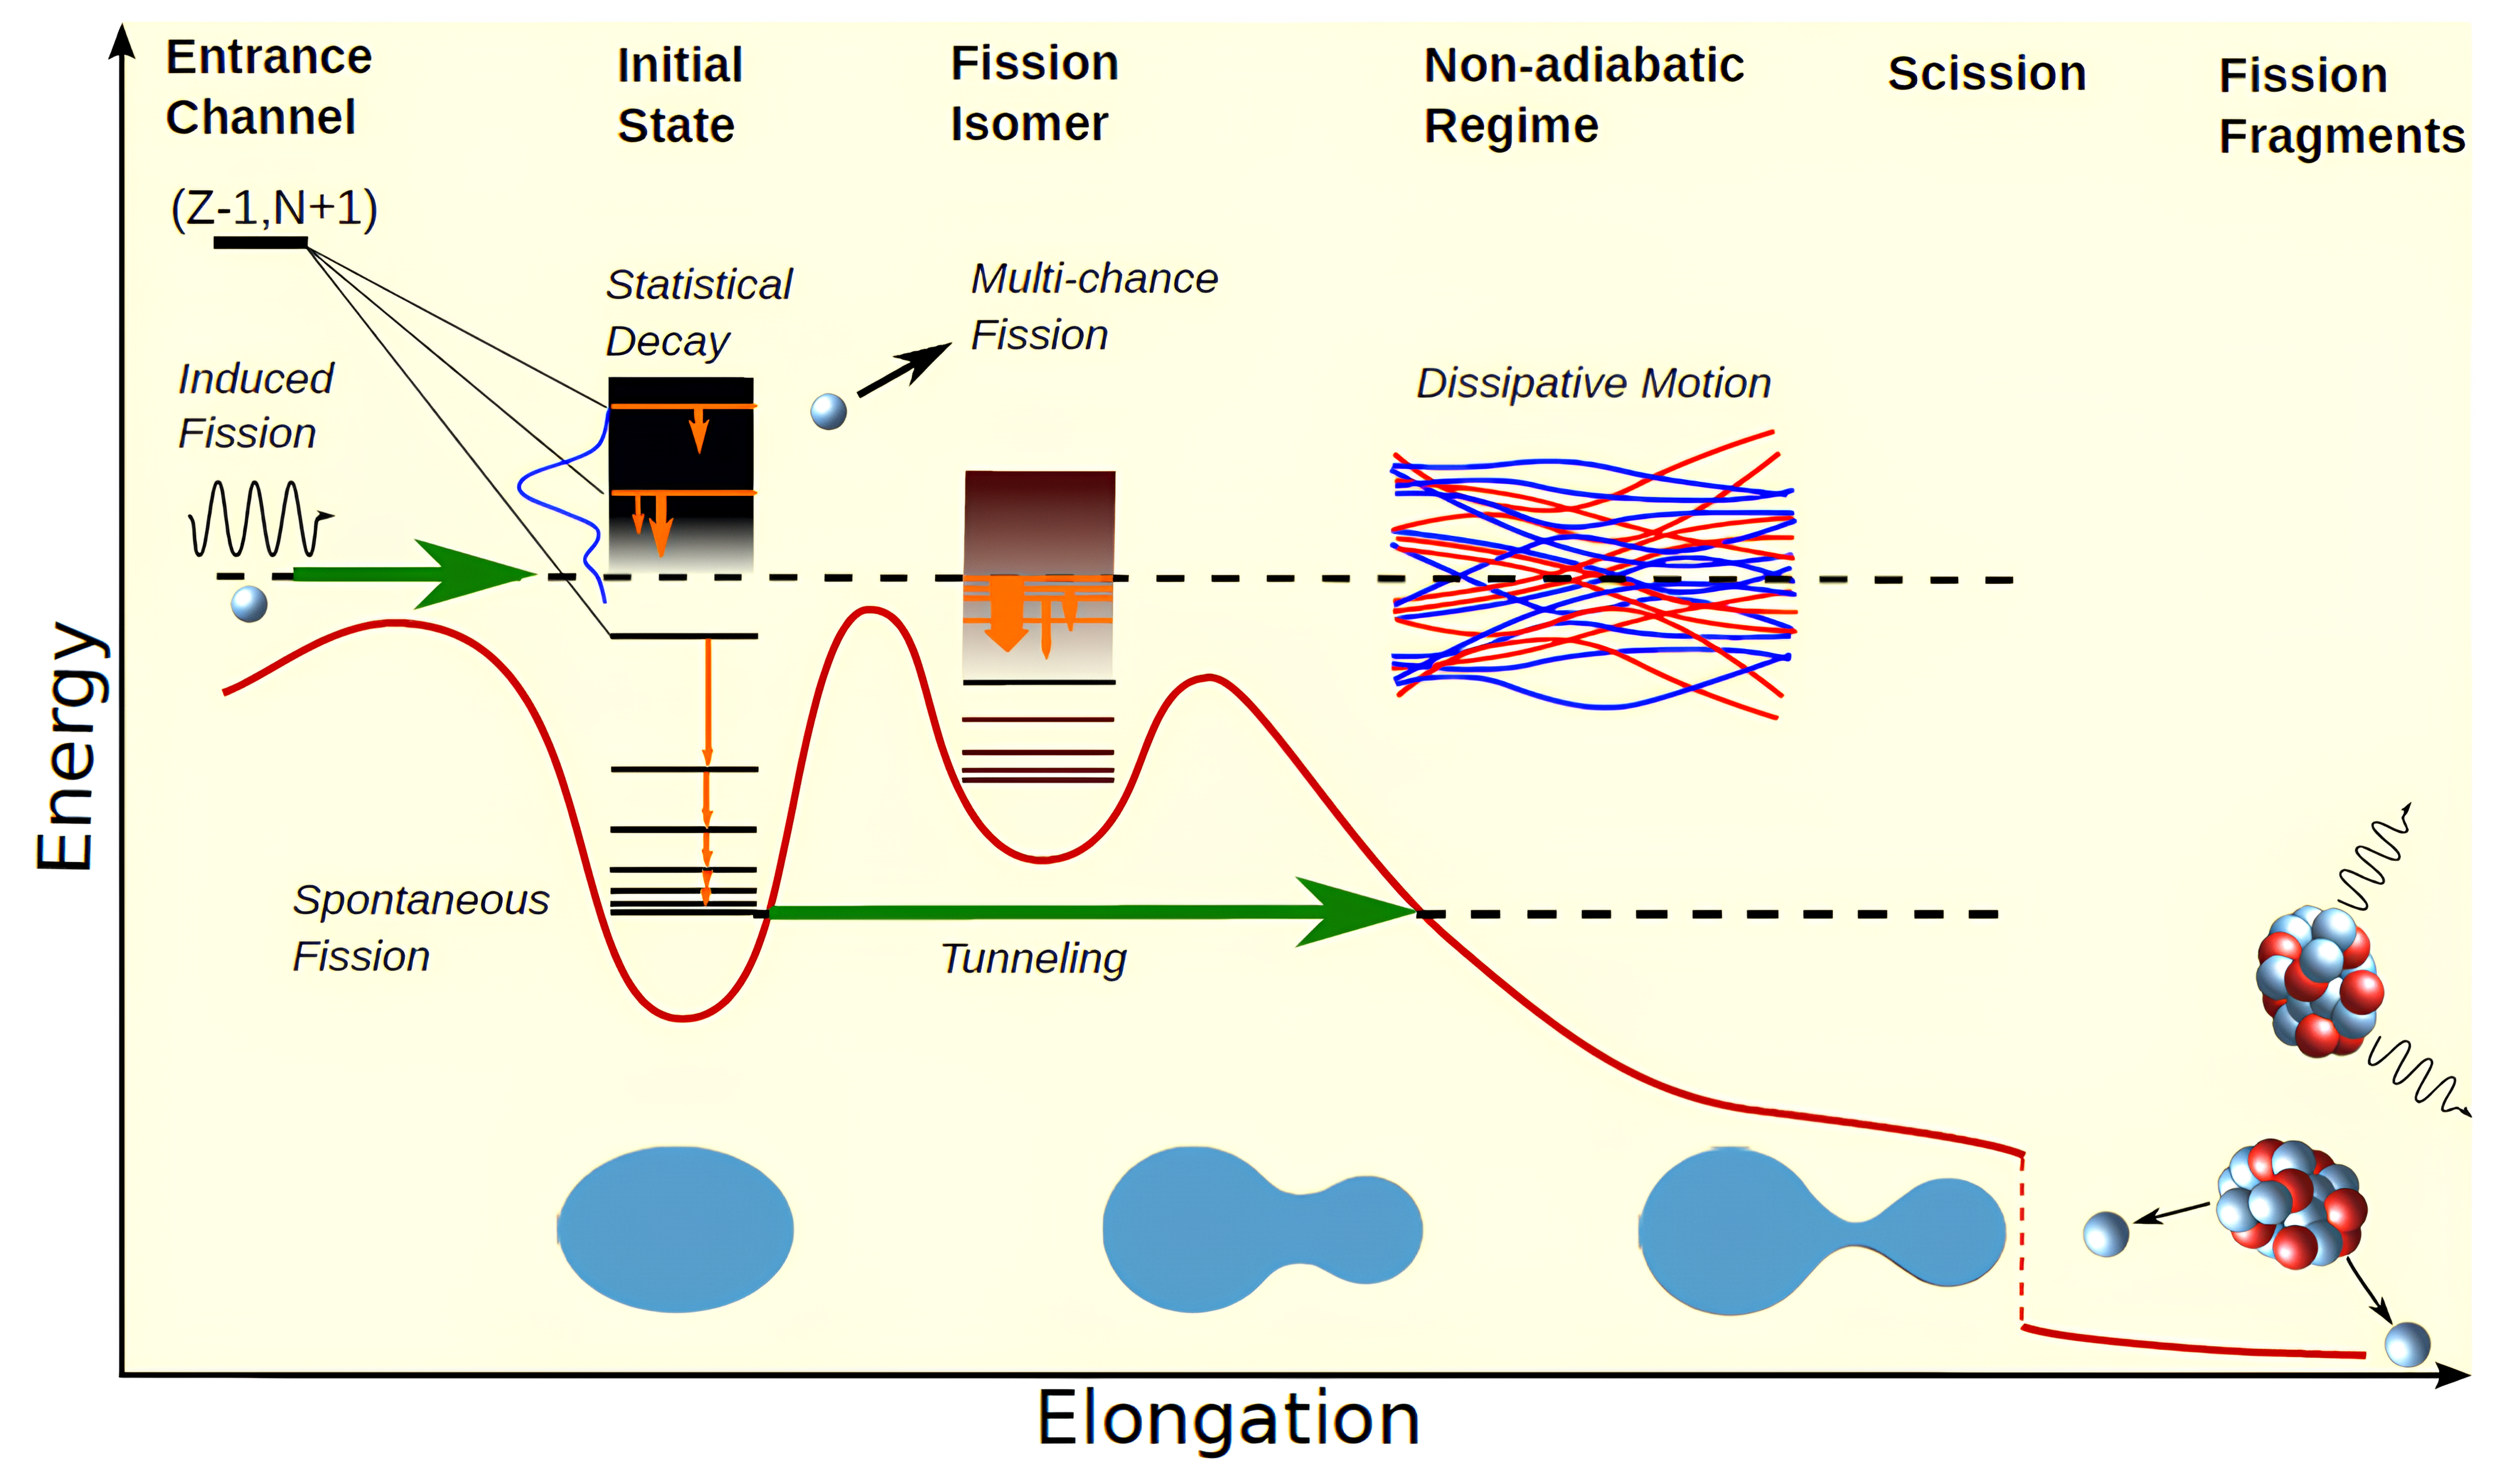
\includegraphics[width=0.85\textwidth]{Images/fission.png}
    \caption{Visual representation of the fission process. Figure taken from \cite{Bender2020}.}
    \label{fig:fission}
\end{figure}

\subsubsection{Spontaneous fission model}
It should be ovious that a formal treatment of deformations and collective modes is necessary to give a theoretical description of fission reactions. We can derive a simple spontaneous fission model by studying the effect of an axial quadrupole deformation on the semiempirical mass formula \ref{eq:semf}.

Let us assume that the nuclear radius may be expanded, as previously done in section \ref{sec:deformations}, as
\begin{equation}
    R = R_0[1+\alpha_{20}Y_{20}].
\end{equation}
Assuming the nuclear volume is conserved across the fission path, the volume energy will not change. As for the surface energy, its variation can be expressed at the lowest order in $\alpha_{20}$ as
\begin{equation}
    \Delta E_\text{surf} = E_\text{surf}
    -E_{0,\text{surf}} = E_{0, \text{surf}}\frac 2 5 \alpha_{20}^2.
\end{equation}
Regarding the Coulomb energy, the variation is given by
\begin{equation}
    \Delta E_\text{coul} = E_\text{coul} - E_{0, \text{coul}} = -E_{0, \text{coul}}\frac 1 5 \alpha_{20}.
\end{equation}
Since the neutron and proton numbers does not change, the surface and Coulomb energies are the only contributions to the total energy difference. We can write
\begin{equation}
    \label{eq:fission_semf}
    \Delta E = \frac 2 5 \alpha_{20}^2 a_s A^{2/3}- \frac 1 5 \alpha_{20}^2 a_c Z^2 A^{-1/3},
\end{equation}
if we set equation \eqref{eq:fission_semf} to zero, we get, other than the undeformed solution for $\alpha_{20}=0$, 
\begin{equation}
    \frac{ Z^2}{A} = \frac{2 a_s}{a_c},
\end{equation}
where the ratio $2a_s/a_c$ amounts to $\approx 50$ in typical parametrizations of the SEMF. Equation \eqref{eq:fission_semf}, shows that for values of the so called \textit{fissility parameter} $Z^2/A$ larger than $50$, the energy change becomes negative, favouring a configuration in which the nucleus fragments due to the spontaneous fission.
\subsection{Symmetry breaking and microscopic approaches to fission}
\subsubsection{Microscopic theory}
The use of phenomenological macroscopic-microscopic models has long provided valuable insight into fission processes, allowing for the prediction of barrier heights and fragment yields through parametrised shape degrees of freedom and empirical shell corrections \cite{Brack1972,Bjornholm1980,Krappe2012}.  
In these models, the total energy is expressed as
\begin{equation}
E_{\mathrm{tot}}(\boldsymbol{q}) = E_{\mathrm{LD}}(\boldsymbol{q}) + \delta E_{\mathrm{shell}}(\boldsymbol{q}) + \delta E_{\mathrm{pair}}(\boldsymbol{q}),
\end{equation}
where $E_{\mathrm{LD}}$ is the macroscopic liquid-drop term depending on deformation coordinates $\boldsymbol{q}$, while $\delta E_{\mathrm{shell}}$ and $\delta E_{\mathrm{pair}}$ account for shell and pairing corrections, respectively.  
While such models reproduce many global observables, they lack a true microscopic foundation.  
In particular, the collective coordinates $\boldsymbol{q}$ are not derived from the underlying many-body dynamics, and the empirical shell corrections cannot describe the self-consistent rearrangement of the mean field along the fission path.

A more fundamental understanding is achieved within self-consistent mean-field approaches such as the Hartree-Fock or Hartree-Fock-Bogoliubov formalisms. The use of nuclear Density Functional Theory \cite{Bender2003,Schunck2016} allows one to define a universal EDF $E[\rho,\kappa]$ that encapsulates both mean-field and pairing correlations.  
The resulting constrained HF/HFB calculations produce the potential energy surface (PES) $E(\boldsymbol{q})$, mapping the energy of the system as a function of collective deformations such as the quadrupole ($Q_{20}$), octupole ($Q_{30}$), and triaxial ($Q_{22}$) moments.  
The minima and saddle points of this multidimensional PES determine the fission barriers and shape isomeric states \cite{Dubray2012,Schunck2016}.

However, static mean-field approaches are limited by their single-reference character: the HFB vacuum represents only one configuration at a time, typically corresponding to a local minimum of the PES.  
In the vicinity of the fission barrier, where several configurations with different intrinsic quantum numbers coexist, this approximation breaks down.  
The wave function should instead be expressed as a superposition of several self-consistent configurations $\{|\Phi(\boldsymbol{q})\rangle\}$, leading to a correlated state of the form
\begin{equation}
|\Psi\rangle = \int f(\boldsymbol{q})\, |\Phi(\boldsymbol{q})\rangle\, d\boldsymbol{q},
\end{equation}
which is the essence of the \emph{Generator Coordinate Method} (GCM) \cite{Goutte2005,Regnier2019}.  
The GCM maps the microscopic many-body problem onto a \emph{collective Schrödinger equation} (CSE)
\begin{equation}
\left[ -\frac{\hbar^2}{2}\sum_{ij}\frac{\partial}{\partial q_i} B_{ij}(\boldsymbol{q}) \frac{\partial}{\partial q_j} + V(\boldsymbol{q}) \right] g_k(\boldsymbol{q})
= E_k g_k(\boldsymbol{q}),
\end{equation}
where $B_{ij}(\boldsymbol{q})$ is the collective inertia tensor and $V(\boldsymbol{q})$ the potential energy extracted from constrained HFB.  
This framework naturally incorporates tunnelling through the barrier and provides access to observables such as fission lifetimes and fragment distributions.  

Beyond-mean-field extensions also restore symmetries that are spontaneously broken at the mean-field level.  
For instance, particle-number, parity, and angular-momentum projection techniques \cite{Bender2004,Samyn2005} are required to recover good quantum numbers and remove spurious symmetry mixing.  
In multi-reference DFT \cite{Bender2003}, these symmetry restorations can be combined with configuration mixing, yielding highly accurate fission barrier calculations.  

\subsubsection{Unconstrained Calculations and Symmetry Breaking}

An equally important aspect of microscopic fission theory is the treatment of spatial symmetries.  
Historically, many calculations imposed constraints such as axial symmetry or reflection symmetry with respect to a plane to reduce the computational cost of solving the HFB equations.  
While such restrictions simplify the description of the nucleus, they artificially constrain the fission path and may even prevent the identification of energetically preferred configurations \cite{Warda2002,Bertsch2018}, as shown in figure \ref{fig:fission_barrier}.  
Fission involves strongly deformed, triaxial, and reflection-asymmetric shapes; the correct description of barrier heights and scission configurations therefore requires breaking as many spatial symmetries as possible.

In the self-consistent mean-field framework, spontaneous symmetry breaking is a feature rather than a flaw: it allows the system to adopt a deformed intrinsic shape corresponding to a broken rotational or parity symmetry, while the symmetry of the total many-body Hamiltonian is preserved.  
For example, an axially deformed HFB state violates rotational invariance, but the restoration of this symmetry through angular-momentum projection recovers the correct laboratory-frame properties.  
Similarly, parity breaking through octupole deformation is essential to describe asymmetric fission fragment distributions. Triaxiality, for example, has been shown to lower the inner barrier of actinides by several MeV \cite{Warda2002,Schunck2016}.
Likewise, reflection-asymmetric (octupole) degrees of freedom are necessary to reproduce mass-asymmetric fission in heavy nuclei.

Recent computational developments have made possible fully symmetry-unrestricted HFB and TDDFT calculations, in which all spatial and time-reversal symmetries can be broken if energetically favourable \cite{Simenel2018,Schunck2016}.  
Codes such as \texttt{HFODD} and \texttt{Sky3D} implement three-dimensional solvers capable of describing triaxial, octupole, and time-odd components of the density matrix.  
These advances have revealed new fission pathways, scission configurations, and fragment-spin correlations inaccessible to axially symmetric models.

In summary, microscopic theories based on DFT and its extensions offer a self-consistent foundation for the description of nuclear fission.  
They provide direct access to the interplay between shell effects, pairing, and deformation, which determine the shape evolution from the ground state to scission.  

\chapter{State of the art, objectives and methods}
\label{chap:methods}
\section{State of the art and motivation}
The need to account for nuclear deformations has been already highlighted as a central theme in Chapter~\ref{chap:intro}, particularly in the context of heavy nuclei and of the complex fission dynamics discussed in Section~\ref{sec:fission}. Without allowing for deformation, several key properties of nuclear systems, such as the rotational bands in the excitation spectrum since spherical nuclei cannot rotate, cannot be captured. Limiting the description to only a subset of shapes, such as axially symmetric configurations, often proves to be inadequate. This is evident in the case of fission dynamics, where the evolution stages happen through very deformed and exotic configurations, explored over relatively long time scales.

The central issue in nuclear structure theory is that the Hamiltonian is not known exactly and must be approximated. At the same time, the problem is inherently a quantum many-body one, which remains computationally demanding, requiring approximations to make calculations tractable. Symmetry assumptions such as spherical or axial symmetry have therefore been widely used in numerical implementations to simplify the calculations and reduce the computational cost. However, these constraints become insufficient in situations where deformation is a defining aspect of the system.

With the increasing availability of computational power and the development of modern numerical techniques, the field is now in a position to move beyond these restrictive assumptions. This motivates the development of new codes capable of treating the many-body problem without imposed symmetries, allowing the full range of nuclear deformations to emerge naturally from the underlying theory.

\section{State of the Art}
The approaches to the nuclear many-body problem can be divided into three families: shell model, ab initio, and Density Functional Theory.
\paragraph{Shell model}
In the interacting shell model, one assumes that a basis is constituted by nucleons in single-particle orbitals. While some orbitals are \emph{frozen}, there is a space called \emph{valence space} in which one includes all possible configurations with nucleons arbitrarily put in the valence orbitals. The nuclear Hamiltonian is diagnonalized in this configuration space. This model is very successful for spectroscopy but also computationally very demanding. Often, the predictive power is srongly dependent on the specific effective Hamiltonian that is assumed.
\paragraph{Ab initio}
One may be inclined towards studying nuclei starting from the fundamental interaction which binds them, the strong force. This would be done starting from the QCD Lagrangian, however, two problems arise. First, nucleons are bound states of quarks and gluons and what binds the nucleus together is the residual interaction arising from these bound systems. Second, the QCD coupling is large at the energy scale $\Lambda_\chi\approx 0.5-1.0$~GeV of nucleons and heavy mesons and as such cannot be treated perturbatively. This is at variance with the higher energy scales like $100-1000$ GeV where QCD is perturbative.

The solution to this problem is the use of effective chiral Lagrangians, equivalent to the QCD one at low energy scales. The interactions among the nucleons arise from the Feynman diagrams between two, three, or more nucleons, which must be hierarchically ordered, according to some perturbative parameter, usually denoted by $(Q/\Lambda_\chi)^\nu$, where $Q$ is the typical nucleon momentum. The power of $\nu$ at which the expansion stops determines the order of the potential that is calculated and used.

These methods are in principle exact, but require nevertheless a series of approximations to make calculations tractable; moreover, their applicability is currently limited to spherical and light deformed nuclei.

\paragraph{Density Functional Theory}
The issues brought forth by the shell model and the ab initio approaches may be addressed by using an \textit{effective} interaction among nucleons that is not derived from exact principles but reliably reproduces experimental data. This was done starting from the 1970s, by minimising the energy functional $\bra{\Psi}\hat{H}_\text{eff}\ket{\Psi}$, where $\hat{H}_\text{eff}$ is a properly designed effective Hamiltonian and $\Psi$ is a Slater determinant.

It was realised early on that the only way to obtain realistic results from this approach was to use density dependent forces, which somewhat account for the important many-body effects. The historical development of this realization has been to first use the Hartree--Fock expectation value of an effective interaction as a starting point for the design of an Energy Density Functional (EDF), which can be used to do nuclear structure calculations using Density Functional Theory. Later, it has been customary to directly write an EDF.

In particular, the minimisation of these EDFs has been done using two numerical approaches: (a) \textit{basis expansion methods}, which represent single-particle states on truncated bases, mainly harmonic oscillator bases, 
and (b) \textit{coordinate-space (mesh) methods}, which discretise space directly by using a mesh. 
In the following sections, we review these two classes of methods and motivate the need for more flexible and computationally efficient unconstrained solvers.

\subsection{Basis expansion methods}

Basis expansion approaches are among the most widely used techniques for solving the HF and HFB equations. 
In these methods, single-particle wavefunctions are expanded on a finite HO basis, chosen for its flexibility and easiness of use, together with the qualitative similarity to the mean-field potential of bound nuclei, as explained in Section~\ref{sec:models}. 
Codes such as \texttt{HFBTHO}, also used in this work for benchmarking our implementation in Section~\ref{sec:hfbtho}, are based on this framework.

The HO basis, although efficient, introduces inherent limitations.
First, weakly bound and continuum-like states, crucial for nuclei near the drip lines, are poorly represented because their asymptotic behaviour differs 
fundamentally from that of HO functions. 
Whereas HO states decay as $e^{-ar^{2}}$, quasi-bound states decay as $e^{-\kappa r}$, 
leading to slow convergence and difficulties in describing haloes, neutron skins, and quasi-resonant states 
\cite{Stoitsov2003_PRCC68_054312,Dobaczewski1996_PRCC53_2809}.  
Second, large deformations in heavy nuclei may require many HO shells to reproduce the stretched spatial geometry, significantly increasing the computational cost.  
The computational complexity grows rapidly with the maximum number of oscillator shells used in the calculation, resulting in demanding memory and CPU requirements for strongly deformed configurations \cite{Marevic2022_CPC}.

In summary, despite their efficiency for near-spherical and moderately deformed nuclei, 
basis-expansion methods become inadequate for describing nuclei near drip lines, far from stability and largely deformed.

\subsection{Symmetry-Restricted mesh methods}

A second major class of HF/HFB solvers uses a spatial mesh.  
Historically, fully unconstrained three-dimensional meshes were computationally prohibitive, which motivated the introduction of \textit{symmetry constraints} to reduce the dimensionality of the problem.  
By enforcing specific spatial symmetries, the number of degrees of freedom is greatly reduced, making coordinate-space calculations tractable on available hardware.

The most common choices are spherical and axial symmetry.  
Spherical HF/HFB solvers \cite{VauhBrinkOriginal,hfbcsqrpa} reduce the equations to a radial problem, achieving excellent computational efficiency and precision for the structure of spherical or near-spherical nuclei.  
Axially symmetric solvers \cite{Pei2008_HFBAX} generalise this approach to two dimensions, allowing axial deformations while still benefitting from significant computational cost reductions.

However, the limitations of symmetry-restricted approaches are inherent to the constraints themselves, as they forbid the emergence of intrinsic shapes such as triaxial or more general octupole-deformed configurations.

\subsection{Unconstrained coordinate-space (mesh) methods}
To overcome the limitations of basis truncation and symmetry constraints, modern HF / HFB solvers have increasingly adopted coordinate-space discretizations, typically based on three-dimensional Cartesian meshes. 
Notable examples include \texttt{MOCCa} \cite{Ryssens2016_MOCCa}, 
\texttt{Sky3D} \cite{Maruhn2014_Sky3D}, and \texttt{HFBFFT} \cite{CHEN2022108344}. 
These codes solve the HF or HFB equations directly in coordinate space, allowing arbitrary deformations and spontaneous symmetry breaking to emerge naturally.

However, coordinate-space solvers come with their own challenges.  
High spatial resolution is required to accomodate sufficient numerical accuracy, leading to large three-dimensional grids, thus substantial computational cost. 
Even with modern resources, fully unconstrained calculations remain computationally intensive, and additional assumptions such as plane reflection symmetry are often introduced to reduce the domain size \cite{Ryssens2015_EV8,Ryssens2016_MOCCa}.
Thus, while mesh-based solvers offer maximal flexibility, their computational demands motivate the search for more efficient numerical approaches.

\subsection{Towards more efficient unconstrained methods}
The limitations discussed above highlight the need for methods that combine the flexibility of coordinate-space solvers with improved computational efficiency.
In this thesis, we investigate such an approach through the use of the \textit{Generalised Conjugate Gradient} (GCG) method, presented in detail in section~\ref{sec:gcg}.
In the HF and energy-density-functional frameworks, the core of the many-body problem reduces to solving a set of single-particle Schrödinger or Kohn--Sham eigenvalue equations, coupled self-consistently through the mean-field.
These equations must be solved repeatedly during the iterative HF/HFB cycle, and their efficient solution dominates the overall computational cost.

As shown in the present work, applying GCG to the HF single-particle problem provides a promising route towards efficient, symmetry-unrestricted many-body calculations while mitigating the main bottlenecks of fully coordinate-mesh methods.

\section{Objectives}
The aim of this work is to develop a new implementation of the Hartree--Fock method on an unconstrained 3D mesh, by the use of the Generalised Conjugate Gradient method. The goals addressed by this work are the following:
\begin{itemize}
    \item demonstrate the feasibility of the Generalised Conjugate Gradient for the solution of large-scale eigenvalue problems;
    \item solve the self-consistent Hartree--Fock equations on an unconstrained 3D mesh;
    \item verify the numerical accuracy of the new implementation, first against existing spherical codes;
    \item second against well-established deformed codes; and
    \item attempt to produce novel results, and establish the advancement brought to the field by this work.
\end{itemize}

\section{Methods}
The methods used in this thesis can be grouped into two main components: the formulation of the Energy Density Functional and the solution of the resulting self-consistent equations.

\paragraph{Skyrme Energy Functional}  
The many-body nuclear problem is approached within the Hartree--Fock framework, described in section~\ref{sec:hf}.  
As discussed in Chapter~\ref{chap:intro}, a pure HF treatment is not sufficient for a quantitative description of nuclear structure, 
and a more general Energy Density Functional (EDF) formulation must be adopted.  
In this work, we employ the Skyrme EDF, whose construction and resulting mean-field equations are developed in section~\ref{sec:skyrme}.  
This provides the self-consistent single-particle Hamiltonian that forms the basis for the numerical treatment.

\paragraph{Finite Differences and Generalised Conjugate Gradient}  
Once the equations to be solved have been derived, their numerical solution requires both a spatial discretization scheme and an efficient solver for the large-scale eigenvalue problem that arises at each iteration of the self-consistent procedure.
Chapter~\ref{chap:numerical} details the methods adopted in this work, starting with the finite-difference discretization of derivatives in section~\ref{sec:finite_diff}.  
The resulting discretised eigenvalue problem is then treated using the GCG method to extract the relevant low-lying eigenstates, as described in section~\ref{sec:gcg}.  
Section~\ref{sec:minimisation} discusses implementation-specific aspects of the code, including convergence criteria, mixing strategies, and the choice of parameters required to ensure stable and efficient minimisation of the energy functional.


\chapter{Energy functional}
\section{Hartree-Fock theory}
An empirical description of nuclear structure can be carried out using phenomenological models, as reported in section (REF).
\\A more rigorous approach needs to take into account the fact that the mean field which the nucleons interact with, is generated by the nucleons themselves, due to some microscopic interaction.
Starting from the many-body hamiltonian of the system, we will be able to extract a single particle hamiltonian, where the nucleon is subject to a mean field potential generated by the effective microscopic force.
\\The many-body hamiltonian of the system, made of $A$ fermions, given by
\begin{equation}
    \label{eq:mb_hamiltonian}
    \hat H = \hat T + \hat V = \sum_i -\frac{\hbar^2}{2m}\nabla^2_i + \sum_{i<j} v^{(2)}_{ij} + \sum_{i<j<k} v^{(3)}_{ijk }+\ldots
\end{equation}
With the Schr\"odinger equation of the many-body system given by
\begin{equation}
    \label{eq:many_body_schrodinger}
    \hat H \Psi = E\Psi.
\end{equation}
\subsection{Variational principle}
Since $\hat H$ is a many body operator, finding its eigenstates would be a rather challenging task. To our aid, comes the variational principle, from which we can show that equation \ref{eq:many_body_schrodinger} is equivalent to 
\begin{equation}
    \label{eq:variational_Psi}
    \delta E[\Psi] = \delta \frac{\bra{\Psi} E \ket{\Psi}}{\bra{\Psi}\ket{\Psi}} = 0.
\end{equation}
The variation \ref{eq:variational_Psi} can be obtained from an arbitrary variation of $\Psi$, which can be done indipendently on $\bra{\Psi}$ and $\ket{\Psi}$, since $\Psi$ is complex, yielding
\begin{equation}
    \label{eq:variational_Psi2}
    \bra{\delta \Psi} \hat H  -E\ket{\Psi} + \bra{\Psi} \hat H-E \ket{\delta \Psi} = 0
\end{equation}
since the variation is arbitrary, we can multiply by a phase factor $\ket{\delta \Psi}\mapsto i\ket{\delta \Psi}$ and get
\begin{equation}
    \label{eq:variational_Psi3}
    -i\bra{\delta \Psi} \hat H-E \ket{\Psi} + i\bra{\Psi} \hat H-E \ket{\delta \Psi} = 0.
\end{equation}
Combining equations \ref{eq:variational_Psi2} and \ref{eq:variational_Psi3}, we get
\begin{equation}
    \label{eq:var_eq_res}
    \bra{\delta \Psi} \hat H-E \ket{\Psi} = 0.
\end{equation}
Again, since the variation is arbitrary, equation \ref{eq:var_eq_res} satisfies equation \ref{eq:many_body_schrodinger}.
\subsubsection{Ground state}
Since we always restrict ourselves to a certain subspace of the full Hilbert space, we can only find an approximate solution to the eigenvalue problem. Expanding this solution on the complete set of exact eigenstates of $\hat H$, we have
\begin{equation}
    \label{eq:expansion_gs}
    \ket\Psi = \sum_n a_n \ket{\Psi_n}    
\end{equation}
the total energy amounts to 
\begin{equation}
    \label{eq:ground_state_min}
    E[\Psi] = \frac{\sum_{nn'}\bra {a_{n'}\Psi_{n'}}\hat H \ket{a_n \Psi_n}}{\sum_{nn'}\bra{a_{n'}\Psi_{n'}}\ket{a_n\Psi_{n}}} = \frac{\sum_{n}E_n|a_n|^2}{\sum_n|a_n|^2}\ge \frac{\sum_{n}E_0|a_n|^2}{\sum_n|a_n|^2}\ge E_0.
\end{equation}
where the orthonormality $\bra{\Psi_{n'}\ket{\Psi_n}}=\delta_{nn'}$ has been used. Equation \ref{eq:ground_state_min} tells us that the minimum of the variational subspace we are considering is bound from below by the true ground state energy.
\subsection{Hartree-Fock equations}
The Hartree-Fock method is the application of the variational principle \ref{eq:var_eq_res} to a many-body wavefunction represented by a Slater determinant, which reads
\begin{equation}
    \label{eq:slater_formula}
    \Psi = \frac{1}{\sqrt {A!}} \sum_{\{p\}} (-1)^{p}  \varphi_{p(1)}(\bm r_1)\ldots \varphi_{p(A)}(\bm r_A)
\end{equation}
where $\varphi_i$ are single-particle states.
The slater determinant sums over all possible permutations of the $A$ fermions on the single particle states, with a $-$ sign according to the parity of the permutation.
The Slater determinant is just the assumption of independent single-particle fermion states, so that the Pauli exclusion principle is not violated.
\\To ensure the orthonormality of the single-particle states, we need to add a Lagrange multiplier to the variation of $E$, which ends up reading
\begin{equation}
    \label{eq:fdv_hf}
\delta \bigg(E[\Psi] - \sum_i\lambda_i \int \varphi_i^*\varphi_i d\bm r \bigg) = 0
\end{equation}
We can explicit $E[\Psi] = \bra{\Psi} \hat T + \hat V\ket \Psi$, which can be expressed using the single-particle states 
\begin{align}
    \label{eq:exp_T_V}
    \bra\Psi\hat T\ket \Psi &= \sum_i^A -\frac{\hbar^2}{2m}\int \varphi_i^*(\bm r) \nabla^2 \varphi_i(\bm r) d\bm r\\
    \bra\Psi\hat V\ket \Psi &= \frac 1 2 \sum_{ij}\int\varphi_i^*(\bm r) \varphi_j^*(\bm r') v_{ij}(\bm r, \bm r')\varphi_i(\bm r)\varphi_j(\bm r') d\bm r d\bm r'\\
    &- \frac 1 2 \sum_{ij}\int \varphi_i^*(\bm r) \varphi_j^*(\bm r') v_{ij}(\bm r, \bm r')\varphi_i(\bm r')\varphi_j(\bm r) d\bm r d\bm r'
\end{align}
If we use $\varphi_i^*(\bm r)$ as the quantity to be varied for equation \ref{eq:fdv_hf}, we get the \textit{Hartree-Fock equations}
\begin{align}
    \label{eq:hf_equations}
    &-\frac{\hbar^2}{2m} \nabla^2 \varphi_i\\
    &+ \sum_{j}^A \int \varphi_j^* (\mathbf r') 
        v_{ij}(\mathbf r, \mathbf r')\, 
        \varphi_j (\mathbf r')\, 
        \varphi_i (\mathbf r)\, d\mathbf r'\label{eq:hartree} \\
    &- \sum_{j}^A \int \varphi_j^* (\mathbf r')\, 
        v_{ij}(\mathbf r, \mathbf r')\,
        \varphi_j (\mathbf r)\,
        \varphi_i (\mathbf r')\, d\mathbf r'\label{eq:fock}
        = \varepsilon_i \varphi_i
\end{align}
here the Lagrange multipliers $\lambda_i$ have been replaced by $\varepsilon_i$, since they can be interpreted as the energy of the single-particle states.\\
Now, a couple of observations are in order.
\paragraph{Exchange interaction}
The interaction term \ref{eq:hartree}, called Hartree term, arises from considering independent particles, and is also routinely found in classical physics. The other one in \ref{eq:fock}, called Fock term, or exchange term, takes the form of an integral operator and is given by the quantum mechanical nature of the problem.
\\For what concerns the solution of equation \ref{eq:hf_equations}, the Fock term is very problematic, and is avoided using finite-range interaction like the Gogny force \cite{Robledo_2019}, or contact forces like the Skyrme one \cite{SKYRME1958615}, which is used in the present work, since they render the exchange term as a local one.
\paragraph{Self-consistent solution}
Even if the interaction terms are local, the equation is still highly non-linear, since the mean field potential will be a function of the eigenfunctions themselves. The consequece is that the solution will be found \textit{self-consistently}, that is, by solving for the set of eigenfunctions $\{\varphi_i\}$, using them to build the new mean field, and solving again, repeating the process until convergence.
\subsection{Symmetries}
Since the objective of this work is to solve the Hartree-Fock equations without spatial symmetry assumptions, it is useful to first understand how symmetries propagate along the self-consistent calculation.
\\We start by defining the creation and annihilation operators of the single particle hamiltonian eigenstates, $a_i^\dagger, a_i$, which abide the usual anticommutation relations of fermions
\begin{equation}
    \label{eq:fermion_anticommutations}
    \{a_i, a_j^\dagger\} = \delta_{ij}
\end{equation}
If we expand on a different, orthonormal complete basis $\{\chi_l\}$, we can write the corresponding creation and annihilation operators $c_l^\dagger, c_l$ as
\begin{align}
    \label{eq:basis_change}
    \varphi_k = \sum_l D_{lk} \chi_l\\
    a_k^\dagger = \sum_l D_{lk} c_l^\dagger\\
    a_k = \sum_l D_{lk}^\dagger c_l
\end{align}
Since orthonormality is guaranteed for both sets, taking 
\begin{equation}
    \delta_{jk} = \bra{\varphi_j}\ket{\varphi_k} = \sum_{ll'} D_{l'j}^\dagger D_{lk}\bra{\chi_l}\ket{\chi_l'}\implies DD^\dagger = 1.
\end{equation}
We can define the density matrix as
\begin{equation}
    \label{eq:density_op}
    \rho_{ll'} = \bra{\Psi}c_{l'}^\dagger c_l\ket{\Psi}
\end{equation}
which in the hartree fock basis, using relations \ref{eq:basis_change}, is diagonal and its trace is equal to the particle number $A$.
\\Writing the many body hamiltonian \ref{eq:many_body_schrodinger} in the arbitrary basis of second quantization operators $c_l^\dagger, c_l$, we get
\begin{equation}
    \label{eq:mb_hamiltonian_sq}
    \hat H = \sum_{l_1 l_2}t_{l_1l_2} c_{l_1}^\dagger c_{l_2} + \frac 1 4 \sum_{l_1 l_2 l_3 l_4}\overline{v}_{l_1l_2l_3l_4} c_{l_1}^\dagger c_{l_2}^\dagger c_{l_3} c_{l_4}
\end{equation}
where $t_{l_1l_2}$ and $\overline{v}_{l_1 l_2 l_3 l_4}$ are defined as 
\begin{align}
    \label{eq:t_op}
    t_{l_1l_2} &= \bra{-}c_{l_1}c_{l_2} t c_{l_1}^\dagger c_{l_2}^\dagger \ket{-} = \bra{l_1 l_2}t\ket{l_1 l_2}
    \\ \overline{v}_{l_1 l_2 l_3 l_4} &= \bra{l_1 l_2 l_3 l_4} v \ket{l_1 l_2 l_3 l_4} - \bra{l_1 l_2 l_4 l_3} v \ket{l_1 l_2 l_4 l_3}
\end{align}
The minimization \ref{eq:fdv_hf} can be restated as the variation of $\bra{\Psi}\hat H \ket{\Psi}$, with respect to the density matrix $\rho_{ll'}$, which yields the single particle hamiltonian $h$
\begin{equation}
    \label{eq:spe_scnd}
    h_{ll'} = \pdv{E[\rho]}{\rho_{ll'}} = t + \sum_{kk'}\overline{v}_{lk'l'k}\rho_{kk'} = t+\Gamma_{ll'}.
\end{equation}
Being $h$ diagonal in the Hartree-Fock basis, the self-consistent solution is the one for which
\begin{equation}
    [h, \rho] = 0
\end{equation}
holds.
\subsubsection{Symmetry propagation}
Suppose to start a Hartree-Fock calculation with an initial guess $\ket{\Psi}^{(0)}$ for which the corresponding density matrix is symmetric under the action of a many-body symmetry operator $S$ which commutes with the Hamiltonian
\begin{equation}
    \label{eq:comm_S_H}
    [S, \hat H] = 0.
\end{equation}
It can be shown \cite{ring2004nuclear} that 
\begin{equation}
    \label{eq:comm_S_Gamma}
    S\Gamma[\rho] S^\dagger  = \Gamma[S\rho S^\dagger].
\end{equation}
The single particle Hamiltonian $h$ will then display the same property
\begin{equation}
    \label{eq:comm_h_S}
    S h[\rho] S^\dagger = h[S\rho S^\dagger]
\end{equation}
meaning that $h$ will be symmetric under the action of $S$, as well as the next iteration's density matrix $\rho^{(1)}$. The symmetry $S$ gets propagated self-consistently until the minimum is found.
\\This has profound numerical implications, since the real minimum of deformed nuclei can be found only starting from starting guesses with similar broken symmetries. It can be the case that numerical noise allows to explore the full energy surface, but if one has to take into consideration the numerical cost of a bad guess, then it's still advantageous to start from a good one.
\subsection{Density Functional Theory}
It shall be evident shortly, in section \ref{sec:skyrme}, that a more general approach to microscopic models has to be taken, in order to give a satisfactory description of the nuclear world.
\\The framework that we'll briefly outline here is called Density Functional Theory (DFT). DFT was introduced by P. Hohenberg and W. Kohn in 1964 \cite{HK}, by proving two theorems.
\\The \textbf{first} HK theorem states that the energy of a fermion system, subject to an external potential $V_\text{ext}$ can be expressed solely as a functional of the particle density $\rho$ of the system.
\begin{equation}
    \label{eq:hk_theorem1}
    E[\rho] = F[\rho] + \int V_\text{ext} \rho(\bm r) d\mathbf r
\end{equation}
While the \textbf{second} one states that the ground state of the system is found by minimizing its variation with respect to $\rho$. 
\\HK theorems are fundamental but not constructive \cite{NDFT}, since they do not provide a form for the functional $F$, which is intrinsic to the physics of the fermions at hand.
COMPLETARE




\section{Skyrme force and functional}
Now that the theoretical framework is clear, we can investigate a plausible nucleonic interaction, which in the present work, takes the form of the Skyrme interaction.
\\It was first proposed by Tony Skyrme in 1958 \cite{SKYRME1958615} as a zero range force between nucleons, and has been used successfully as the building block of theoretical nuclear structure.
\\Nowadays, the standard form is slightly enriched to be more general \cite{CHABANAT1997710}. It comprises a two-body interaction, which reads
\begin{align*}
v^{(2)}(\mathbf{r}_1, \mathbf{r}_2) &= t_0 \left(1 + x_0 P_\sigma \right) \delta(\mathbf{r}) \\
&\quad + \frac{1}{2} t_1 \left(1 + x_1 P_\sigma \right) \left[ \mathbf{P}'^2 \delta(\mathbf{r}) + \delta(\mathbf{r}) \mathbf{P}^2 \right] \\
&\quad + t_2 \left(1 + x_2 P_\sigma \right) \mathbf{P}' \cdot \delta(\mathbf{r}) \mathbf{P} \\
&\quad + \frac{1}{6} t_3 \left(1 + x_3 P_\sigma \right) \left[ \rho(\mathbf{R}) \right]^\sigma \delta(\mathbf{r}) \\
&\quad + i W_0 \boldsymbol{\sigma}\cdot \left[ \mathbf{P}' \times \delta(\mathbf{r}) \mathbf{P} \right]
\end{align*}
And a three body interaction, that is
\begin{equation*}
v^{(3)}(\mathbf r_1, \mathbf r_2)=\frac 1 6 t_3 \left(1 + x_3 P_\sigma \right) \left[ \rho(\mathbf{R}) \right]^\sigma \delta(\mathbf{r}) 
\end{equation*}
Where 
\begin{align*}
\\\mathbf{r} &= \mathbf{r}_1 - \mathbf{r}_2
\\\mathbf{R} &= \frac{\mathbf{r}_1+\mathbf{r}_2}{2}
\\\mathbf{P} &= \frac{-i(\nabla_1 - \nabla_2)}{2}
\\\boldsymbol{\sigma} &= \boldsymbol{\sigma}_1 + \boldsymbol{\sigma}_2
\\\mathbf{P}_\sigma &= \frac{(1+\boldsymbol{\sigma}_1\cdot\boldsymbol{\sigma}_2)}{2}
\end{align*}
Primed operators refer to the adjoint operator acting on the dual space.
\\This formulation respects all symmetries required of a non relativistic nuclear interaction 
\begin{itemize}
    \item Galilean boost
    \item Particle exchange
    \item Translation
    \item Rotation
    \item Parity
    \item Time reversal
\end{itemize}
The zero-range characteristic takes the form of a Dirac delta $\delta(\mathbf r)$, which allows to write the exchange Fock term detailed in (REF) as a local one.
\\Taking the expectation value of the many body hamiltonian, in the Hilbert space of Slater determinants, yields
\begin{equation}
    \label{eq:slater_exp}
    \expval{H} = \bra{\Psi} H \ket{\Psi} = \int (\mathcal E_\text{Skyrme} + \mathcal E_\text{Kin}) d\mathbf r = \int \mathcal E d\mathbf r
\end{equation}
Since the Skyrme interaction is time-reversal invariant (as well as the kinetic operator), this means that the total Hamiltonian must be time-even.
Different additive contributions must be time-even as well, even if the densities from which they are calculated are not. Unless we reduce to the even-even nucleus case, where total angular momentum is defined at $J=0$, giving vanishing time-odd densities.
This allows us to write the functional in a simpler form as \cite{stevenson2019low}
\begin{align}
    \mathcal E_\text{Kin} &= \frac{\hbar^2}{2m}\tau \label{eq:kinfunc}\\
    \mathcal E_\text{Skyrme} &= \sum_{t=0,1}\bigg\{C_t^\rho [\rho_0]\rho_t^2+C_t^{\Delta \rho}\rho_t\nabla^2\rho_t+C_t^{\nabla\cdot J}\rho_t\nabla\cdot \mathbf J_t + C_t^\tau\rho_t\tau_t\bigg\}\label{eq:skfunc}
\end{align}
Here, $t=0,1$ refers to the isoscalar and isovector components of the densities, e.g.
\begin{align*}
    \rho_0 = \rho_p + \rho_n
    \\\rho_1 = \rho_p - \rho_n
\end{align*}
Where
\begin{align}
    \label{eq:coefficients_func}
    C_0^\rho &= +\frac 3 8 t_0 + \frac 3 {48} t_3\rho_0^\sigma 
    \\C_1^\rho &= -\frac 1 8 t_0(1+2x_0)- \frac 1 {48} t_3(1+x_3)\rho_0^\sigma 
    \\C_0^\tau &= +\frac 3 {16} t_1 + \frac 1 {16} t_2 (5+4x_2)
    \\C_1^\tau &= -\frac 1 {16} t_1(1+2x_1)+\frac 1 {16}t_2(1+2x_2)
    \\C_0^{\Delta \rho} &= -\frac 9 {64}t_1+\frac 1 {64}t_2(5+4x_2)
    \\C_1^{\Delta \rho} &= +\frac 3 {64}t_1(1+2x_1)+\frac 1 {64}t_2(1+2x_2)
    \\C_0^{\nabla\cdot J} &= -\frac 3 4 W_0
    \\C_1^{\nabla\cdot J} &= -\frac 1 4 W_0
\end{align}
As outlined in previous chapters (REF), we can now derive the Kohn-Sham equations, by constraining orthonormality and enforcing the variation of the functional to be zero. What we end up with is
\begin{equation}
    \label{eq:spe_ks}
    \bigg[-\nabla\bigg(\frac{\hbar^2}{2m^{*}_q(\mathbf r)}\nabla \bigg) + U_q(\mathbf r) + \delta_{\text{q,proton}}U_C(\mathbf r)-i\mathbf B_q(\mathbf r)\cdot(\nabla \times \boldsymbol\sigma) \bigg]\varphi_\alpha=\varepsilon_\alpha\varphi_\alpha
\end{equation}
The index $q=n,p$ refers respectively to the neutron and proton quantities.
\\Where the different terms are given by
\begin{align}
    \frac{\hbar^2}{2m^{*}_q(\mathbf r)} &= \fdv{\mathcal E}{\tau_q}
    \\U_q(\mathbf r) &= \fdv{\mathcal E}{\rho_q}\label{eq:fdv_rho_skyrme}
    \\\mathbf B_q(\mathbf r) &= \fdv{\mathcal E}{\boldsymbol{\mathbf J_q}}
\end{align}
The coulomb field $U_C$, which is present only in the single particle equation for protons, doesn't come from the skyrme interaction, rather from the Coulomb part of the whole functional. It will be properly derived in section \ref{sec:coulomb_treatment}.
\\Following the rules for functional derivatives, outlined in the appendix (REF) we get
\begin{align}
    \frac{\hbar^2}{2m_q^*(\mathbf r)} =& +\frac{\hbar^2}{2m} \\&+ \frac 1 8 [t_1(2+x_1)+t_2(2+x_2)]\rho(\mathbf r) \\&- \frac 1 8 [t_1(1+2x_1)+t_2(1+2x_2)]\rho_q(\mathbf r ) \\\\
    U_q(\mathbf r) =& +\frac 1 8 [t_1(2+x_1)+t_2(2+x_2)]\rho \\&+ \frac 1 8 [t_2(1+2x_2)-t_1(1+2x_1)]\rho_q \\
    &+ \frac 1 8 [t_1(2+x_1)+t_2(2+x_2)]\tau \\&+ \frac 1 8 [t_2(1+2x_2)-t_1(1+2x_1)]\tau_q \\
    &+ \frac 1 {16} [t_2(2+x_2)-3t_1(2+x_1)] \nabla^2 \rho \\&+ \frac 1 {16} [3t_1(2x_1+1)+t_2(2x_2+1)] \nabla^2 \rho_q \\\\
    \mathbf W_q (\mathbf r ) = &+\frac 1 2 W_0 [\nabla\rho + \nabla \rho_q] \\&-\frac 1 8 (t_1 x_1 + t_2 x_2) \mathbf J + \frac 1 8 (t_1 - t_2) \mathbf J_q 
\end{align}
Unless otherwise specified, unindexed densities denote isoscalar quantities (sum of neutron's and proton's).
\subsection{Energy density functional}
The energy functional to be minimised is of the form \cite{Bender2003}
\begin{equation}
\label{eq:full_functional}
E_{\text{HF}} =  E_\text{Kin}+E_\text{Skyrme}+E_\text{Coul} = \int( \mathcal E_\text{Kin} + \mathcal E_\text{Skyrme} + \mathcal E_\text{Coul})d\bm r.
\end{equation}
\subsubsection{Densities}
Functional \eqref{eq:full_functional} can be expressed through a series of generlized particle densities. Let us define them and express them on the spin coordinates up ($\uparrow$) and down ($\downarrow$) for the convenience in a mesh representation.
\\The starting point is the density matrix, defined as
\begin{equation}
    \rho_q (\mathbf r \sigma, \mathbf r \sigma') = \sum_{\alpha} \phi_{\alpha, \sigma} (\mathbf r )\phi_{\alpha, \sigma'}^*(\mathbf r')
\end{equation}
where the index $\alpha$ goes through all single particle states of the particles of type $q$ (protons, neutrons) and the index $\sigma$ refers to the spin coordinate. The particle density is defined as 
\begin{align}
    \rho_q(\mathbf r) \coloneq\rho_q(\mathbf r, \mathbf r')\bigg|_{\mathbf{r} = \mathbf{r'}} \coloneq \sum_{\sigma}\rho(\mathbf r\sigma, \mathbf r'\sigma) \bigg|_{\mathbf{r} = \mathbf{r'}} &=\sum_{\alpha} \phi_{\uparrow}(\mathbf r)\phi_{\uparrow}^*(\mathbf r')+\phi_{\downarrow}(\mathbf r)\phi_{\downarrow}^*(\mathbf r') \bigg|_{\mathbf{r} = \mathbf{r'}} \nonumber
    \\&=\sum_{\alpha} |\phi_{\uparrow}(\mathbf r)|^2+|\phi_{\downarrow}(\mathbf r)|^2.
    \label{eq:part_density}
\end{align}
The kinetic density reads
\begin{align}
    \tau_q(\mathbf r) &\coloneq \sum_{\alpha} \nabla'\cdot\nabla\rho_q(\mathbf r, \mathbf r')\bigg|_{\mathbf r'=\mathbf r} \nonumber
    \\&= \sum_{\sigma, \alpha} \nabla \phi_\sigma (\mathbf r)\cdot \nabla \phi_\sigma^*(\mathbf r')\bigg|_{\mathbf r = \mathbf r'} = \sum_{\sigma, \alpha} |\nabla \phi_\sigma(\mathbf r)|^2 \nonumber
    \\&= \sum_{\alpha}|\nabla \phi_\uparrow(\mathbf r)|^2 + |\nabla \phi_\downarrow(\mathbf r)|^2 \label{eq:kin_density}.
\end{align}
The spin density  reads
\begin{align}
    s_q(\mathbf r, \mathbf r') &\coloneq\sum_{\sigma \sigma', i} \rho_q(\mathbf r \sigma, \mathbf r' \sigma')\bra{\sigma'} \hat {\boldsymbol{\sigma}} \ket{\sigma} = \sum_{\alpha} \begin{bmatrix} \phi_{\uparrow}^*(\mathbf r') \ \phi_{\downarrow}^*(\mathbf r') \end{bmatrix}\hat{\boldsymbol{\sigma}} \begin{bmatrix} \phi_{\uparrow}(\mathbf r) \\ \phi_{\downarrow}(\mathbf r) \end{bmatrix}
\end{align}
and lastly, the spin-orbit density tensor reads
\begin{align}
    J_{q, \mu\nu} &\coloneq \frac 1 {2i}(\partial_\mu - \partial_\mu') s_{q, \nu}(\mathbf r, \mathbf r')\bigg|_{\mathbf r'=\mathbf r}\nonumber \\
    &= \frac 1 {2i}\bigg(\begin{bmatrix}\phi_{\uparrow}^*(\boldsymbol r')\ \phi_{\downarrow}^*(\boldsymbol r')\end{bmatrix} \partial_\mu\hat{\sigma}_\nu\begin{bmatrix} \phi_{\uparrow}(\mathbf r) \\ \phi_{\downarrow}(\mathbf r) \end{bmatrix} - \begin{bmatrix}\phi_{\uparrow}(\boldsymbol{r})\ \phi_{\downarrow}(\boldsymbol{r})\end{bmatrix} \partial_\mu'\hat{\sigma}_\nu\begin{bmatrix} \phi_{\uparrow}^*(\mathbf r') \\ \phi_{\downarrow}^*(\mathbf r') \end{bmatrix}\bigg)_{\mathbf r'=\mathbf r}\nonumber
     \\&= \sum_\alpha\Im\bigg\{\begin{bmatrix}\phi_{\uparrow}^*(\boldsymbol r)\ \phi_{\downarrow}^*(\boldsymbol r) \end{bmatrix}\partial_\mu \hat{\sigma}_\nu\begin{bmatrix} \phi_{\uparrow}(\mathbf r) \\ \phi_{\downarrow}(\mathbf r) \end{bmatrix}\bigg\}
\end{align}
which also defines the spin-orbit current vector $\bm J$ that reads
\begin{equation}
     J_{q,\kappa} (\bm r ) = \sum_{\mu\nu}\epsilon_{\kappa\mu\nu} J_{q, \mu\nu}(\bm r).
\end{equation}
\subsubsection{Kinetic functional}
The kinetic term can be expressed as
\begin{equation}
    \label{eq:kinfunc}
    \mathcal E_\text{Kin} = \frac{\hbar^2}{2m}\tau
\end{equation}
which is found integrating by parts \eqref{eq:kin_functional}.
\subsubsection{Skyrme functional}
Since this work only deals with even-even nuclei, only time-even densities, which are the ones previously defined, are non-vanishing, due to the ground state being time-reversal invariant \cite{Bender2003}. This reduces the Skyrme functional to the following form \cite{stevenson2019low}
\begin{align}
    \label{eq:skfunc}
    \mathcal E_\text{Skyrme} &= \sum_{t=0,1}\bigg\{C_t^\rho [\rho_0]\rho_t^2+C_t^{\Delta \rho}\rho_t\nabla^2\rho_t+C_t^{\nabla\cdot J}\rho_t\nabla\cdot \mathbf J_t + C_t^\tau\rho_t\tau_t\bigg\}
\end{align}
where
\begin{align}
    %\label{eq:coefficients_func}
    C_0^\rho &= +\frac 3 8 t_0 + \frac 3 {48} t_3\rho_0^\sigma \label{eq:C0rho}
    \\C_1^\rho &= -\frac 1 8 t_0(1+2x_0)- \frac 1 {48} t_3(1+x_3)\rho_0^\sigma \label{eq:C1rho}
    \\C_0^\tau &= +\frac 3 {16} t_1 + \frac 1 {16} t_2 (5+4x_2) \label{eq:C0tau}
    \\C_1^\tau &= -\frac 1 {16} t_1(1+2x_1)+\frac 1 {16}t_2(1+2x_2) \label{eq:C1tau}
    \\C_0^{\Delta \rho} &= -\frac 9 {64}t_1+\frac 1 {64}t_2(5+4x_2) \label{eq:C0Deltarho}
    \\C_1^{\Delta \rho} &= +\frac 3 {64}t_1(1+2x_1)+\frac 1 {64}t_2(1+2x_2) \label{eq:C1Deltarho}
    \\C_0^{\nabla\cdot J} &= -\frac 3 4 W_0 \label{eq:C0nabladotJ}
    \\C_1^{\nabla\cdot J} &= -\frac 1 4 W_0 \label{eq:C1nabladotJ}.
\end{align}
Here, $t=0,1$ refers to the isoscalar and isovector components of the densities, that is
\begin{align*}
    \rho_0 = \rho_p + \rho_n
    \\\rho_1 = \rho_p - \rho_n
\end{align*}
and the same holds for all generalised densities.
We can now derive the Kohn-Sham equations, by minimising the functional under the constraint
\begin{equation}
    \label{eq:spe_ks_constraint}
    \bra{\varphi_i}\ket{\varphi_j}=\delta_{ij}.
\end{equation}
The resulting Kohn-Sham equations are of the form
\begin{equation}
    \label{eq:spe_ks}
    \bigg[-\nabla\bigg(\frac{\hbar^2}{2m^{*}_q(\mathbf r)}\nabla \bigg) + U_q(\mathbf r) + \delta_{\text{q,proton}}U_C(\mathbf r)-i\mathbf B_q(\mathbf r)\cdot(\nabla \times \boldsymbol\sigma) \bigg]\varphi_\alpha=\varepsilon_\alpha\varphi_\alpha
\end{equation}
where an effective mass field arises, which is defined as
\begin{equation}
    \frac{\hbar^2}{2m^{*}_q(\mathbf r)} = \fdv{\mathcal E}{\tau_q}
\end{equation}
a mean field potential, which reads
\begin{equation}
    U_q(\mathbf r) = \fdv{\mathcal E}{\rho_q}\label{eq:fdv_rho_skyrme}
\end{equation}
and a spin-orbit field, given by
\begin{equation}
    \label{eq:sofield}
    \mathbf B_q(\mathbf r) = \fdv{\mathcal E}{\boldsymbol{\mathbf J_q}}.
\end{equation}
The coulomb field $U_C$, which is present only in the single particle equation for protons, doesn't come from the Skyrme interaction, rather from the Coulomb part of the whole functional. It will be properly derived in section \ref{sec:coulomb_treatment}.
\\Following the rules for functional derivatives, outlined in the appendix \ref{app:func_der} we get
\begin{align}
    \frac{\hbar^2}{2m_q^*(\mathbf r)} =& +\frac{\hbar^2}{2m} \nonumber
    \\&+ \frac 1 8 [t_1(2+x_1)+t_2(2+x_2)]\rho(\mathbf r) \nonumber
    \\&- \frac 1 8 [t_1(1+2x_1)+t_2(1+2x_2)]\rho_q(\mathbf r ) \\\nonumber
\end{align}
\begin{align}
    U_q(\mathbf r) =& +\frac 1 8 [t_1(2+x_1)+t_2(2+x_2)]\rho \nonumber
    \\&+ \frac 1 8 [t_2(1+2x_2)-t_1(1+2x_1)]\rho_q \nonumber
    \\&+ \frac 1 8 [t_1(2+x_1)+t_2(2+x_2)]\tau \nonumber
    \\&+ \frac 1 8 [t_2(1+2x_2)-t_1(1+2x_1)]\tau_q \nonumber
    \\
    &+ \frac 1 {16} [t_2(2+x_2)-3t_1(2+x_1)] \nabla^2 \rho \nonumber
    \\&+ \frac 1 {16} [3t_1(2x_1+1)+t_2(2x_2+1)] \nabla^2 \rho_q \\\nonumber
\end{align}
\begin{align}
    \mathbf B_q (\mathbf r ) = &+\frac 1 2 W_0 [\nabla\rho + \nabla \rho_q] \nonumber\\
    &-\frac 1 8 (t_1 x_1 + t_2 x_2) \mathbf J + \frac 1 8 (t_1 - t_2) \mathbf J_q.
\end{align}
Unless otherwise specified, unlabelled densities denote isoscalar quantities (sum of neutron and proton).
\subsection{Functionals}
The set of parameters $(t_0, t_1, t_2, t_3, x_0, x_1, x_2, \sigma, W_0)$ in the Skyrme functional \eqref{eq:skfunc} is not universal and varies between different parametrisations. These parameters are fitted to experimental data so that the resulting EDF can reproduce known nuclear properties with good accuracy. 

The last widely used family of Skyrme forces derived directly from an effective interaction is the SLy series, which was primarily fitted to properties of magic nuclei and to constraints from neutron-rich matter in neutron stars \cite{chabanat2}. Subsequently, the development of new parametrisations has been driven by the need to reproduce more accurately the masses and radii of nuclei across the nuclear chart, including open-shell and deformed systems. Notable examples include the classic SIII force \cite{Beiner1974}, the deformation-oriented SkM* parametrisation \cite{Bartel1982} to accurately reproduce the $^{240}$Pu fission barrier, and modern large-scale optimisations such as UNEDF0 \cite{KortUNEDF0}.
\section{Coulomb interaction}
\label{sec:coulomb_treatment}
Unlike the Skyrme interaction, the Coulomb force is not local, giving rise to an unwanted integral operator in the Hamiltonian.
A well known and widely used device is the Slater approximation \cite{SlaterApp}, which gives a local exchange interaction.
\\In this approximation, the Coulomb energy reads
\begin{align*}
    E_\text{Coul} = \int \mathcal E_\text{Coul}(\mathbf r) d\bm r
    \\\mathcal E_\text{Coul}(\bm r) = \frac{e^2}{2}\bigg[\int  \frac{\rho_p(\mathbf r )\rho_p(\mathbf r ' )}{|\mathbf r-\mathbf r'|}d\mathbf r'  - \frac 3 2 \bigg(\frac 3 \pi \bigg) ^{\frac 1 3}\rho_p^{4/3}(\mathbf r)\bigg]
\end{align*}
Which gives
\begin{equation}
    U_{C}(\mathbf r) = \fdv{\mathcal E_\text{Coul}}{\rho_p} = \frac{e^2}{2}\bigg[\int \frac{\rho_p(\mathbf r ')}{|\mathbf r-\mathbf r'|} d^3 \mathbf r' - 2\bigg(\frac 3 \pi \bigg) ^{\frac 1 3} \rho_p^{1/3}(\mathbf r ) \bigg]
\end{equation}
From a computational standpoint, the exchange part is trivial, while the direct one is more involved.
One could compute the integral, but the complexity on a 3D mesh is $\mathcal O(N^6)$, rendering it unusable for fine meshes.
\\An alternative approach is to solve the poisson equation (from now on, $V_c$ refers to the direct part only)
\begin{equation}
    \label{eq:poisson}
    \nabla^2 V_c = 4\pi e^2 \rho_p
\end{equation}
Given the proton density, we can impose Dirichlet boundary conditions, which can be extracted from a quadrupole expansion of the charge density \cite{Jackson1998}
\begin{equation}
V_c (\mathbf r) = 4\pi e^2 \sum_{\lambda=0}^2\sum_{\mu=-\lambda}^\lambda \frac{\expval{Q_{\lambda\mu}} Y_{\lambda\mu}}{r^{1+\lambda}}\text{ on }\partial \Omega
\end{equation}
Where $\expval{Q_{\lambda\mu}}$ is defined as 
\begin{equation}
    \expval{Q_{\lambda\mu}} = \int r^\lambda Y_{\lambda\mu}^* (\mathbf r)\rho_p(\mathbf r ) d^3 \mathbf r
\end{equation}
Since we expect a charge density confined to the nuclear shape, higher order terms in the expansion can be neglected, provided that the box is sufficiently large.
\\In a reference frame where the nucleus center of mass is at the origin, the expansion reduces to
\begin{equation}
    V_{c}(\mathbf r ) = \frac{Ze^2}{r} + e^2\sum_{\mu=-2}^{2}\frac{\expval{Q_{2\mu}}Y_{2\mu}}{r^3} \text{ on } \partial \Omega
\end{equation}
Refer to appendix \ref{sec:spherical_harmonics} for the definition and numerical evaluation of the spherical harmonics $Y_{\lambda\mu}$.
\section{Energy calculation}
One, if not the most important physical quantity we want to compute is the total energy of the system.
\\The obvious way would be to evaluate the functinal for a given density. We will call this \textit{integrated energy}.
\begin{align}
    E_\text{int} = E[\rho, \tau, J_{\mu\nu}]= \int \mathcal E d\mathbf r
\end{align}
An alternative approach is to realize that, in a stationary point $\delta E = 0$, the single particle eigenvalue equation stands true
\begin{align}
    \label{eq:simple_spe}
    (\hat t + U)\varphi_k = \varepsilon_k \varphi_k
\end{align}
We can multiply \ref{eq:simple_spe} on the left by $\varphi_k^*$ and integrate to get
\begin{align}
    \label{eq:int_simple_spe}
    \int -\varphi_k^* \frac{\hbar^2}{2m}\nabla^2\varphi_k d\bm r + \int \varphi_k^* U \varphi_k d\bm r = \int \varphi_l^* \varepsilon_k \varphi_k d\bm r
\end{align}
The integral on the right hand side of \ref{eq:int_simple_spe} evaluates to $\varepsilon_k$ due to the orthonormality constraint. If we sum over all states $k$ we get
\begin{align}
    \sum_k \bigg\{\int -\varphi_k^* \frac{\hbar^2}{2m}\nabla^2\varphi_k d\bm r + \int \varphi_k^* U \varphi_k d\bm r \bigg\}= \sum_k \varepsilon_k 
    \\\sum_k t_k + \int \rho U = \sum_k \varepsilon_k \label{eq:sum_spe}
\end{align}
Since $U$ is calculated as \ref{eq:fdv_rho_skyrme}, assuming that the functional has a power dependence from $\rho$ of the form $\mathcal E = A\rho^{\sigma+1}$ as in our case, we get the \textit{rearrangement energy}
\begin{align}
    \label{eq:sum_spe_new}
    \rho U = \rho \fdv{\mathcal E}{\rho} = \rho(\sigma +1)A \rho^\sigma = (\sigma+1)A \rho^{\sigma+1} = \mathcal E + \sigma \mathcal E = \mathcal E + \mathcal E_\text{rea}
\end{align}

Given the energy of the total system from \ref{eq:slater_exp}, we have
\begin{align}
\sum_k t_k + \frac 1 2 \int \mathcal E d\bm r = E
\end{align}
If we explicit $\mathcal E$ in equation \ref{eq:sum_spe} using \ref{eq:sum_spe_new}, we finally get to
\begin{align}
    \int \mathcal Ed\bm r = \sum_k (\varepsilon_k -t_k) - \sigma\int \mathcal Ed\bm r
\end{align}
Substituting it in equation \ref{eq:sum_spe_new} yields
\begin{align}
    \label{eq:hf_energy}
E_\text{HF} = \frac 1 2 \sum_k (\varepsilon_k + t_k) - \sigma \int \mathcal E d\bm r = \frac 1 2 \bigg(T+\sum_k\varepsilon_k\bigg) +E_\text{rea}
\end{align}
Which will be called \textit{Hartree-Fock energy} throughout this text.
\subsubsection{Sidenote: actual calculation}
As shown in \ref{eq:coefficients_func}, the actual functional has a plethora of $\rho$ terms, which can be summarized as
\begin{equation}
    \mathcal E = \sum_j A_j \rho^{\sigma_j+1} \implies E_\text{rea} = -\sum_j \sigma_j A_j \rho^{\sigma_j+1} 
\end{equation}
This means that only terms with a $\sigma_j\neq 1, -1$ actually contribute to the rearrangement energy.
\\Since equation \ref{eq:hf_energy} is valid only in the minimum of the functional, it's useful in Hartree-Fock calculations to check its equivalence with the integrated energy, so one can be sure to actually be in a minimum.
\chapter{Numerical methods}
This chapter is devoted to describing the practical implementation of the nuclear Hartree-Fock method of this work. In section \ref{sec:finite_diff}, the two partial differential equations (PDEs) of interest, the Kohn-Sham equation and the Poisson equation, are numerically approximated through finite differences. In section \ref{sec:eigensolvers}, a breakdown of numerical solvers for the large-scale eigenvalue problem posed by the KS equation is presented, to didactically illustrate the reason and implementation of the GCG algorithm. Finally, in section \ref{sec:minimization}, the self-consistent calculation is presented, along with the implementation of spatial constraints and the optimization of the numerical parameters of GCG.
\section{Finite differences}
One, if not the easiest way to numerically represent and solve differential equations, is through finite differences. The core idea is to find a suitable 3D mesh for the problem at hand, use an approximation for derivatives on said mesh, and ultimately using the language of linear algebra to formulate and solve the resulting system of equations.
\subsection{3D mesh}
The first task on the agenda, is finding a suitable representation of the various fields for a computer.
Generally speaking, we deal at most with 2-rank tensors, which vary in space and spin. 
\\Discretizing the 3D cartesian space with a 3-index mesh, choosing a box which size on x, y, z is respectively $[-a_x, a_x]$, $[-a_y, a_y]$, $[-a_z, a_z]$, and a number of points $N_x, N_y, N_z$, the resulting lattice will be given by
\begin{equation*}
V=\{(-a_x+ih_x, -a_y+ih_y, -a_z+ih_z)\} = \{(x_i, y_j,z_k)\} 
\end{equation*}
Where the indices and step size are
\begin{align*}
  i&=0,\ldots,N_x-1,\ h_x = \frac{2a_x}{N_x-1}\\
  j&=0,\ldots,N_y-1,\ h_y = \frac{2a_y}{N_y-1}\\
  k&=0,\ldots,N_z-1,\ h_z = \frac{2a_z}{N_z-1}
\end{align*}
For ease of notation, we will assume $a=a_x=a_y=a_z=a$ and $N=N_x=N_y=N_z=N$, without losing generality.
\\Including the spin degree of freedom, we can finally represent fields in a numerical way through
\begin{equation}
    \psi(\bm r, \sigma) \mapsto \psi(x_i, y_j, z_k, s) = \psi_{ijks}
\end{equation}
\subsubsection{Discretizing differential operators}
By using Taylor series, it's possible to write approximations to derivatives \cite{Zhou1993}, in any point of the lattice, of any (reasonable) order of accuracy, involving only near neighbouring points. In the present work, 5-points derivates are used, meaning Taylor expansions are written for $\psi(x\pm h)$ and $\psi(x\pm 2h)$ to compute the differential operators. Formulae for first and second derivates in this framework are given in appendix \ref{app:5p_derivatives}.
\subsection{Schr\"odinger equation}
As outlined in (REF), one of the two PDEs we want to solve is the single particle Schr\"odinger equation \ref{eq:spe_ks}.
\\It can be summarized as
\begin{equation}
    \label{eq:pde} f(\nabla^2 \psi, \nabla \psi, \psi, \bm r, s) = E\psi
\end{equation}
If $f$ is linear in $\psi$, it would be possible to employ the powerful numerical methods of linear algebra to solve the problem.
Breaking down each part of the equation, the kinetic term
\begin{equation}
\label{eq:kin_lin_dim}
\nabla\bigg(\frac{\hbar^2}{2m^{*}_q(\mathbf r)}\nabla \bigg)\psi = \frac{\hbar^2}{2m^{*}_q(\mathbf r)} \nabla^2\psi + \nabla\bigg(\frac{\hbar^2}{2m^{*}_q(\mathbf r)}\bigg) \nabla\psi
\end{equation}
Is evidently linear in $\psi$. 
\\The spin-orbit coupling, which most generally reads
\begin{align*}
    \hat {{h}}_{\text{SO}}&=\bm f (\bm r )\cdot (\nabla \times \pauli ) 
    \\&=f_x(\bm r)(\sigma_z\partial_y - \sigma_y\partial_z) + f_y(\bm r)(\sigma_x\partial_z - \sigma_z\partial_x) + f_z(\bm r)(\sigma_y\partial_x - \sigma_x\partial_y)
\end{align*}
where $\hat {h}_\text{SO}$ acts linearly on the spinor $\psi_{ijk}$.
Finally, the mean field terms $U_q, U_c$ are just multiplicative, hence linear in $\psi$.
\begin{equation*}
    U\psi
\end{equation*}
Given that the whole equation is linear in $\psi$, we can evaluate it on the chosen mesh, using finite differences to approximate the differential operators, yielding a linear system of equations of the form
\begin{align}
    \sum_n^{N_x\cdot N_y\cdot N_z \cdot 2} A_{mn}\psi_{n} &= E\psi_m
\end{align}
\subsubsection{Boundary conditions}
We expect the nucleus to be a localized object, prompting for null Dirichlet boundary conditions for the Schr\"odinger equation.
Near the boundaries, the derivatives will involve points outside the box. Setting these points to zero, is equivalent to solving 
\begin{equation}
    \begin{bmatrix}
        0 & 0 & 0 & 0 & 0
        \\0 & 0 & 0 & 0 & 0
        \\0 & 0 & A & 0 & 0
        \\0 & 0 & 0 & 0 & 0
        \\0 & 0 & 0 & 0 & 0
    \end{bmatrix}
    \begin{bmatrix}
        \psi_{-2}\\\psi_{-1}\\\psi\\\psi_{N}\\ \psi_{N+1} 
    \end{bmatrix}
    = E 
    \begin{bmatrix}
        \psi_{-2}\\\psi_{-1}\\\psi\\\psi_{N}\\ \psi_{N+1} 
    \end{bmatrix}
\end{equation}
From this system of equations, we get for points outside the boundary:
\begin{equation}
    \begin{cases}
        \psi_{-2} = 0\\
        \psi_{-1} = 0\\
        \ldots
    \end{cases}
\end{equation}
Meaning that $\psi$ outside the box will automatically be set to zero if the $A$ matrix is built assuming those points to be zero.
\subsection{Poisson equation}
\label{subsec:poisson}
The other fundamental PDE we need to solve is the Poisson equation encountered in section (REF). Dropping the $c$ and $p$ subscripts, it reads
\begin{equation*}
\nabla^2 V = 4\pi e^2 \rho
\end{equation*}
It's much simpler than the Schr\"odinger equation, as it only involves a laplacian and it is not an eigenvalue problem. The right is side is given, and the solution is found by inverting the matrix.
\subsubsection{Boundary conditions}
Unlike the Schr\"odinger equation, we do not expect the solution to rapidly decay near the boundaries; as reported in section \ref{sec:coulomb_treatment}, we have fixed, non-null boundary conditions, which we have to properly impose on the system.
\\We can choose a direction, say $x$, and look at the equation at the boundaries $x=\pm a$. Since the indeces $j,k$ won't vary, we can omit them, and ignore the other derivates in the following equations.
\begin{align}
    \label{eq:poisson_disc}
    \nabla^2 V = \partial_{xx} V + \partial_{yy}V + \partial_{zz}V = \frac{-V_{i-2} + 16V_{i-1} -30V_i + 16V_{i+1} - V_{i+2}}{12h^2}+\cdots=4\pi e^2 \rho_i
\end{align}
Near a boundary, say $i = 0$, the formula calls for points outside the box, known as \textit{ghost points}. Since they are not part of the linear system, but they are known, we can bring them on the right side of equation \ref{eq:poisson_disc}.
\begin{align}
    \frac{-30 V_0 + 16 V_1 - V_2 }{12h^2} &= 4\pi e^2 \rho_0 +\frac{ V_{-2} -16V_{-1}}{12h^2} = \tilde\rho_0
\end{align}
The same procedure must be applied to all equations involving ghost points, e.g. for $i=1$
\begin{align}
    \frac{+16V_0 -30V_{1} + 16 V_2 - V_3}{12h^2} &= 4\pi e^2 \rho_1 + \frac{V_{-1} }{12h^2} = \tilde\rho_1
\end{align}
The proper system to solve will then be
\begin{align}
A V = \tilde \rho
\end{align}
Where $A$ is constructed as previously specified. $\tilde \rho $ will force the solution to abide boundary conditions.
\subsubsection{On higher order approximations and performance}
Higher and higher order approximations for derivatives involve points that are further and further away. This increases accuracy, but it also decreases matrix sparseness.
\\Algorithms like Conjugate Gradient, as we'll see in the next section,  and linear algebra computing libraries, benefit from matrix sparseness. The implication is that performance \textit{vs} accuracy is a tradeoff that isn't univocal to every problem.
\\In the present work, the golden choice has been 5-point stencils; but it's not definitive, as the lattice points rapidly cap depending on the system's memory.
\\As an example, take a seemingly harmless grid, made of 50 points in each direction. The resulting matrix will be $50\times 50 \times 50 \times 2=\num{2.5e5}$ both in columns and rows. 
It may be the case in the future, that higher order derivatives will be needed, to compensate for the limitation brought by the $\mathcal O (h^n)$ polynomial accuracy of the method in the step size.
\section{Conjugate gradient methods}
This section is devoted to exploring the idea behind the Conjugate Gradient (CG) algorithm and its use in the General Conjugate Gradient (GCG).
\subsection{Conjugate Gradient}
The CG method is used for solving linear systems of the form
\begin{equation}
    \label{eq:lin_sys}
    Ax = b
\end{equation}
Where $A$ is an $n\times n$ matrix, and $x$ and $b$ are $n$-dimensional vectors.
\\The quadratic form $f(x)$ associated to this system  
\begin{equation}
    \label{eq:quad_form}
    f(x) = \frac 1 2 x^T A x - b^T x
\end{equation}
If $A$ is symmetric, positive-definite, the 



\section{Code implementation details}
\subsection{Constraints}
\label{sec:alm}
The purpose of spatial constraints is to find the minimum of the energy functional under the condition that the expectation value of a given operator $\mathcal Q$ equals a prescribed target value $q_0$.
Constrained calculations are a fundamental tool to assess the stability of the ground-state minimum and to investigate dynamical properties of the nucleus, such as fission barriers \cite{bonche1985self}.
\\Constraints can be formulated as an equality-constrained optimization problem (ECP), formulated as
\begin{align}
\min_{\ket \Psi}&E 
\\\text{constrainted to } &\bra{\Psi} {\mathcal Q} \ket {\Psi} = \expval{ {\mathcal Q}} = q_0
\end{align}
Which yields the Lagrangian
\begin{equation}
    \label{eq:constr_lagrangian}
    E' = E + \lambda (\expval{{\mathcal Q}}-q_0)
\end{equation}
where $\lambda$ is a Lagrange multiplier determined by the condition $\expval {{\mathcal Q}} = q_0$. 
After finding the minimum of $E'$, it's trivial to show that for a given $\lambda$, we get \cite{FLOCARD1973433}
\begin{equation}
\dv{E}{\expval{{\mathcal Q}}} = -\lambda. 
\end{equation}
From a numerical standpoint, $\lambda$ needs to be tuned at each iteration to reach the desired value of $q_0$. 
This method was the one used in early constrained Hartree-Fock calculations \cite{Cusson1985}.
\\Although this method is simple, it often fails. Moreover, for the same value of $\lambda$, many, possibly infinite values of $\expval{{\mathcal Q}}$ can be obtained, for which we are only allowed to get the one with the most stable solution.
\\A different method is provided by the Quadratic Penalty Method (QPM). Briefly speaking, instead of a Lagrange multiplier, we add a quadratic contribution to the functional, such that
\begin{equation}
    \label{eq:constr_quadratic}
    E' = E + \frac c 2 (\expval{{\mathcal Q}}-q_0)^2.
\end{equation}
This is a straightforward method; intuitively one penalizes (hence the name), any solution for which $\expval{{\mathcal Q}}\neq q_0$ by increasing its energy. However, the success of such procedure is heavily influenced by the choice of $c$, often leading to instabilities for large values.
\\What happens is that for small values of $c$, the penalty may be insufficient to reach the target $q_0$, while for bigger values, the penalty may be so strong that the self-consistent calculation oscillates and fails.
\subsubsection{Augmented Lagrangian Method}
A modern, robust approach, used by HF/HFB codes \cite{RYSSENS2015175,CHEN2022108344} is given in the form of the Augmented Lagrangian Method (ALM) \cite{Staszczak2010}.
Its main idea is to combine the precision of the ECP with the accuracy of the QPM.
\\Without delving into cumbersome mathematical details, we'll see how the algorithm is practically implemented in the code.
\\Given the functional
\begin{equation}
    \label{eq:alm_lagrangian}
    E' = E + \lambda (q-q_0) + \frac c 2 (q-q_0)^2
\end{equation}
where $q = \expval{{\mathcal Q}}$, the resulting mean field potential will be given by
\begin{align}
    U' &= U + \lambda  {\mathcal Q} + c(q-q_0) {\mathcal Q} 
    \\ &= U + c(q-q_0(\lambda)) {\mathcal Q}
\end{align}
where $q_0(\lambda)$ is updated at each iteration with the formula
\begin{align}
    \label{eq:alm_q0}
    q_0(\lambda) = q_0 - \frac{\lambda}{c}
    \\\lambda ^{(i+1)} = \lambda^{(i)}+\mu c(q-q_0)
\end{align}
Here, a slight deviation from the original ALM is present. Since the original work \cite{Staszczak2010} doesn't provide guidance regarding what is considered an \textit{iteration}, we employ the strategy \cite{CHEN2022108344} of using a damping factor $\mu\in [0, 1]$, so $\lambda$ can be updated at each HF iteration for fast convergence, without large oscillations or instabilities of any kind.
\\This method is what powers the deformation curves that are shown in section (REF), allowing to explore the energy surface with arbitrary precision in reaching the value of $q_0$ at convergence, provided that enough HF iterations are performed.
\\Note that, since $\lambda^{(0)}=0$, for $\mu=0$ ALM reduces to the standard QPM.


\subsection{Self consistent procedure pseudocode}
\chapter{Results for spherical nuclei}
In this chapter, results for spherical nuclei are presented. These are mostly calculated for double magic nuclei, with the exception of $^{90}$Zr.
The reason behind choosing spherical nuclei as an initial benchmark, is that numerous spherical HF codes are available and they have the advantage of being one-dimensional, which allows the use of very fine meshes, with a step size that can go down to the physical scale of the problem, which is roughly 0.1 fm in this case, without any major computational limit. We can use these codes as a reference ideal value for the different quantities produced by our code. The choice for benchmarking spherical results in the present work has been the \texttt{hfbcs\_qrpa} code \cite{hfbcsqrpa}.
\section{Physical quantities}
After finding a nuclide's ground state, we are able to compute different physical properties of the system. We can use these values as a numerical reference when comparing our results with other codes.
\subsection{Mean square radii}
An important set of quantities characterizing the nuclear density is certainly the one of mean square radii.
The individual nuclear spieces' mean square radius is defined as
\begin{equation}
    \label{eq:msr}
    \expval{r^2_q} = \frac{\int\rho_q(\bm r) r^2 d\bm r}{\int \rho_q(\bm r) d\bm r}.
\end{equation}
While the charge mean square radius formula is derived from the convolution of the neutron and proton particle densities with their respective internal charge distribution \cite{BERTOZZI1972408}, resulting in equation \ref{eq:cmsr}.
\begin{equation}
    \label{eq:cmsr}
    \expval{r^2_{ch}} = \expval{r^2_p} + \expval{r^2}_P + \frac N Z \expval{r^2}_N + \frac 2 Z \bigg(\frac{ \hbar}{mc}\bigg)^2\sum_{\alpha q}\mu_q \expval{\bm \sigma\cdot \bm {\ell}}_{\alpha q}
\end{equation}
where $q$ runs over the nuclear species and $\alpha$ runs over all single particle states of spcies $q$. $\bm \sigma$ is the vector operator of Pauli matrices, while $\bm {\ell}$ is the angular momentum operator $-i(\bm r \times \nabla)$.
$\expval{r^2}_P$ and $\expval{r^2}_N$ refer to the square charge radii of the proton and the neutron, while $\mu_q$ to their respective magnetic dipole moment in units of nuclear magneton.
\\All square charge radii computed in this work use the set of parameters in table \ref{tab:charge_par}.
\begin{table}[ht]
  \centering
  \begin{tabular}{lcc}
    \toprule
    \textbf{Parameter} & \textbf{Value} & \textbf{Units} \\
    \midrule
    $\expval{r^2}_P$ & 0.64 & fm$^2$ \\
    $\expval{r^2}_N$ & -0.11 & fm$^2$ \\
    $\mu_p$ & 2.792847 & - \\
    $\mu_n$ & -1.913043 & - \\
    \bottomrule
  \end{tabular}
  \caption{Parameters used to compute the charge mean square radius}
  \label{tab:charge_par}
\end{table}
\subsection{Deformation parameters}
When dealing with deformed nuclei, mean square radii are not sufficient to characterize the nuclear density. The main parameter used is the quadrupole deformation parameter $\beta_2$, defined already in section (REF), it can be computed through the actual mean square radius with formula \ref{eq:beta_real_radius}
\begin{equation}
    \label{eq:beta_real_radius}
    \beta_2 = \frac{4\pi\expval{Y_{2 0}}}{3A\expval{r^2}}
\end{equation}
where $\expval{r^2}$ is the total mean square radius of the nucleus 
\begin{equation}
    \expval{r^2} = \frac{\int (\rho_n + \rho_p )r^2 d\bm r}{\int (\rho_n + \rho_p )d\bm r} = \expval{x^2+y^2+z^2}.
\end{equation}
For spherical nuclei, $\beta_2 = 0$, while for deformed ones, thanks to the normalization with respect to the total radius and mass, the $\beta_2$ parameter can be used to compare different nuclei across the nuclide chart.
\section{Parameters and mesh choice}
\label{sec:hfbcs}
All $\texttt{hfbcs\_qrpa}$ calculations were performed using a mesh size of $0.1$ fm, no pairing interaction, and a radial mesh size whose radius is equal to the side of the box in our computation. The lattice of our code depends on the extension of the nucleus, which is directly determined by its mass $A$; since the number of subdivisions that allows reasonable CPU times on a laptop caps around $60-70$, step sizes vary across different calculations. 
In the results shown here, for $^{16}$O, we are able to reach a $0.3$ fm step size, while for the heaviest, $^{90}$Zr, we are only able to reach $0.42$ fm. The reason behind this choice is that as the nucleus size increases, a bigger box is needed to ensure that all relevant states are able to decay to zero at the boundary. All the data reported in this chapter is computed with the SLy5 parametrization \cite{chabanat2}.
\section{Results for \(^{16}\)O}
\label{sec:oxygen}
The first results we will take a look at are the ones for $^{16}$O. It is an ideal benchmark for gauging the solver's performance, as it is a very light, double magic nucleus, meaning it has no pairing interaction and a spherical shape.
All calculations are performed on a box of size $[-9, 9]$ fm in all three directions and a step size of $0.3$ fm, corresponding to $2\cdot 60^{3}$ mesh points.
\subsection{Results neglecting Coulomb interaction}
Since the Skyrme functional is complex and nuanced, results are shown for more and more terms in expression \eqref{eq:skfunc}. We start by including only $C_0^\rho$, $C_1^\rho$, $C_0^\tau$, $C_1^\tau$ and neglecting the others, and the Coulomb interaction; results are reported in table \ref{tab:no_so_no_j_no_coul}.
Without further terms, the spin-orbit field $\bm B(\bm r)$ vanishes, hence the $1p_{3/2}$ and $1p_{1/2}$ levels show degeneration in energy.

Since $N=Z$, assuming equal masses the single-particle equations will be exactly equal between the two species, therefore only neutron results are reported. Note that $C_1$ terms vanish in this case, that is until we either break the $N=Z$ equality or introduce the Coulomb interaction.
\begin{table}[ht]
  \centering
  \begin{tabular}{lrrccc}
    \multicolumn{6}{c}{\textbf{Physical quantities}}\\
    \addlinespace[0.3em]
    \toprule
    && GCG & hfbcs\_qrpa & $\Delta$ & $\Delta\%$ \\
    \midrule
    $E_{\text{TOT}}$& [MeV] & -141.582 & -141.582 & - & - \\
    $\expval{ r^2_n}^{1/2}$ &[fm] & 2.6504 & 2.6510 & 0.0006 & \num{2.26e-2}\\
    $\expval{ r^2_{ch}}^{1/2}$ &[fm] & 2.7486 & 2.7491 & 0.0005 & \num{1.82e-2}\\
    \midrule
    \addlinespace[1.3em]
    \multicolumn{6}{c}{\textbf{Neutron energy levels}}\\
    \addlinespace[0.3em]
    \midrule
    && GCG & hfbcs\_qrpa & $\Delta$ & $\Delta\%$ \\
    \midrule
    1s$_{1/2}$ &[MeV] & -36.142 & -36.139 & 0.003 & \num{8.30e-3}\\
    1p$_{3/2}$ &[MeV] & -18.573 & -18.572 & 0.001 & \num{5.38e-3}\\
    1p$_{1/2}$ &[MeV] & -18.573 & -18.572 & 0.001 & \num{5.38e-3}\\
    \bottomrule
  \end{tabular}
  \caption{$^{16}$O including $C_0^{\rho}$, $C_1^{\rho}$, $C_0^{\tau}$, $C_1^{\tau}$ terms, neglecting Coulomb interaction.}
  \label{tab:no_so_no_j_no_coul}
\end{table}

In table \ref{tab:compare_so} the $C_0^{\div \bm J}$ and $C_1^{\div \bm J}$ terms are included just for the spin-orbit field $\bm B(\bm r)$, but not for the mean field $U(\bm r)$; from an interaction point of view, it is as if we were neglecting the $J^2$ terms in the energy density \cite{chabanat2}. As expected, the $1p_{3/2}$ and $1p_{1/2}$ degeneration is removed, displaying the spin-orbit splitting, which lowers the total angular momentum $j=3/2$ level and raises the $j=1/2$ level.

\begin{table}[ht]
  \centering
  \begin{tabular}{lrrccc}
    \multicolumn{6}{c}{\textbf{Physical quantities}}\\
    \addlinespace[0.3em]
    \toprule
    && GCG & hfbcs\_qrpa & $\Delta$ & $\Delta\%$ \\
    \midrule
    $E_{\text{TOT}}$& [MeV] & -142.080 & -142.080 & - & - \\
    $\expval{ r^2_n}^{1/2}$ &[fm] & 2.6516 & 2.6516 & - & -\\
    $\expval{ r^2_{ch}}^{1/2}$ &[fm] & 2.7497 & 2.7497 & - & -\\
    \midrule
    \addlinespace[1.3em]
    \multicolumn{6}{c}{\textbf{Neutron energy levels}}\\
    \addlinespace[0.3em]
    \midrule
    && GCG & hfbcs\_qrpa & $\Delta$ & $\Delta\%$ \\
    \midrule
    1s$_{1/2}$ &[MeV] & -36.314 & -36.312 & 0.002 & \num{5.5e-3}\\
    1p$_{3/2}$ &[MeV] & -20.696 & -20.696 & - & -\\
    1p$_{1/2}$ &[MeV] & -14.335 & -14.335 & - & -\\
    \bottomrule
  \end{tabular}
  \caption{$^{16}$O including $C_0^\rho$, $C_1^\rho$, $C_0^\tau$, $C_1^\tau$, $C_0^{\div \bm J}$, $C_1^{\div \bm J}$ terms, neglecting Coulomb interaction and $J^2$ terms.}
  \label{tab:compare_so}
\end{table}

Lastly, the $C_0^{\div \bm J}$ and $C_1^{\div \bm J}$ terms are also included in the calculation of the mean-field, resulting in the full implementation of the Skyrme functional. As shown in table \ref{tab:compare_j2}, the effect of this addition on the ground state is little, as the spin current $J_{\mu \nu}$ is small in light, closed shell nuclei.

\begin{table}[ht]
  \centering
  \begin{tabular}{lrrccc}
    \multicolumn{6}{c}{\textbf{Physical quantities}}\\
    \addlinespace[0.3em]
    \toprule
    && GCG & hfbcs\_qrpa & $\Delta$ & $\Delta\%$ \\
    \midrule
    $E_{\text{TOT}}$& [MeV] & -142.074 & -142.074 & - & - \\
    $\expval{ r^2_n}^{1/2}$ &[fm] & 2.6515 & 2.6516 & 0.0001 & \num{3.77e-3}\\
    $\expval{ r^2_{ch}}^{1/2}$ &[fm] & 2.7497 & 2.7497 & - & -\\
    \midrule
    \addlinespace[1.3em]
    \multicolumn{6}{c}{\textbf{Neutron energy levels}}\\
    \addlinespace[0.3em]
    \midrule
    && GCG & hfbcs\_qrpa & $\Delta$ & $\Delta\%$ \\
    \midrule
    1s$_{1/2}$ &[MeV] & -36.309 & -36.308 & 0.001 & \num{2.75e-3}\\
    1p$_{3/2}$ &[MeV] & -20.684 & -20.685 & 0.001 & \num{4.83e-3}\\
    1p$_{1/2}$ &[MeV] & -14.361 & -14.361 & - & -\\
    \bottomrule
  \end{tabular}
  \caption{$^{16}$O neglecting Coulomb interaction.}
  \label{tab:compare_j2}
\end{table}
\subsubsection{Results including Coulomb interaction}
As the final addition to get a complete and accurate description of $^{16}$O, the Coulomb interaction is included as detailed in section \ref{sec:coulomb_treatment}. Results are shown in table \ref{tab:confronto}.
\begin{table}[ht]
  \centering
  \begin{tabular}{lrrccc}
    \multicolumn{6}{c}{\textbf{Physical quantities}}\\
    \addlinespace[0.3em]
    \toprule
    && GCG & hfbcs\_qrpa & $\Delta$ & $\Delta\%$ \\
    \midrule
    $E_{\text{TOT}}$& [MeV] & -128.402 & -128.400 & 0.002 & \num{1.56e-3} \\
    $\expval{ r^2_n}^{1/2}$ &[fm] & 2.6584 & 2.6585 & 0.0001 & \num{3.76e-3}\\
    $\expval{ r^2_p}^{1/2}$ &[fm] & 2.6835 & 2.6836 & 0.0001 & \num{3.73e-3}\\
    $\expval{ r^2_{ch}}^{1/2}$ &[fm] & 2.7805 & 2.7803 & 0.0002 & \num{7.19e-3}\\
    \midrule
    \addlinespace[1.3em]
    \multicolumn{6}{c}{\textbf{Neutron energy levels}}\\
    \addlinespace[0.3em]
    \midrule
    && GCG & hfbcs\_qrpa & $\Delta$ & $\Delta\%$ \\
    \midrule
    1s$_{1/2}$ &[MeV] & -36.140 & -36.137 & 0.003 & \num{8.30e-3}\\
    1p$_{3/2}$ &[MeV] & -20.611 & -20.611 & - & -\\
    1p$_{1/2}$ &[MeV] & -14.427 & -14.428 & 0.001 & \num{6.93e-3}\\
    \midrule
    \addlinespace[1.3em]
    \multicolumn{6}{c}{\textbf{Proton energy levels}}\\
    \addlinespace[0.3em]
    \midrule
    && GCG & hfbcs\_qrpa & $\Delta$ & $\Delta\%$ \\
    \midrule
    1s$_{1/2}$ &[MeV] & -32.349 & -32.345 & 0.004 & \num{1.24e-2}\\
    1p$_{3/2}$ &[MeV] & -17.137 & -17.137 & - & -\\
    1p$_{1/2}$ &[MeV] & -11.081 & -11.082 & 0.001 & \num{9.02e-3}\\
    \bottomrule
  \end{tabular}
  \caption{$^{16}$O complete of the Skyrme functional and Coulomb interaction.}
  \label{tab:confronto}
\end{table}
\\As shown in tables \ref{tab:no_so_no_j_no_coul}, \ref{tab:compare_so}, \ref{tab:compare_j2}, and \ref{tab:confronto} results for $^{16}$O are in great agreement with the output of the \texttt{hfbcs\_qrpa} code for all the terms in the energy functional.
\section{Results for heavier nuclei}
\label{sec:heavier}
In the following section, results for some spherical nuclei heavier than $^{16}$O are presented.
$^{48}$Ca in table \ref{tab:compare_all_ca48}, $^{56}$Ni in table \ref{tab:compare_all_ni56}, and $^{90}$Zr in table \ref{tab:compare_all_zr90}.
Our code still shows good agreement with the \texttt{hfbcs\_qrpa} one. A slight increase of the numerical error can be observed as the step size increases, which is compatible with the polynomial error in the finite difference method. The increase of the cubic box size is necessary to accomodate larger nuclei, due to the increase in volume occupied, as to guarantee that less bound states decay to zero at the boundary.
\begin{table}[ht]
  \centering
  \begin{tabular}{lrrccc}
    \multicolumn{6}{c}{\textbf{Physical quantities}}\\
    \addlinespace[0.3em]
    \toprule
    && GCG & hfbcs\_qrpa & $\Delta$ & $\Delta\%$ \\
    \midrule
    $E_{\text{TOT}}$& [MeV] & -415.955 & -415.931 & 0.024 & \num{5.77e-3} \\
    $\expval{ r^2_n}^{1/2}$ &[fm] & 3.6106 & 3.6110 & 0.0004 & \num{1.11e-2}\\
    $\expval{ r^2_p}^{1/2}$ &[fm] & 3.4502 & 3.4507 & 0.0005 & \num{1.45e-2}\\
    $\expval{ r^2_{ch}}^{1/2}$ &[fm] & 3.5274 & 3.5060 & 0.0214 & 0.610\\
    \midrule
    \addlinespace[1.3em]
    \multicolumn{6}{c}{\textbf{Neutron energy levels}}\\
    \addlinespace[0.3em]
    \midrule
    && GCG & hfbcs\_qrpa & $\Delta$ & $\Delta\%$ \\
    \midrule
    1s$_{1/2}$ &[MeV] & -49.758 & -49.752 & 0.006 & \num{1.21e-2}\\
    1p$_{3/2}$ &[MeV] & -35.952 & -35.949 & 0.003 & \num{8.34e-3}\\
    1p$_{1/2}$ &[MeV] & -33.891 & -33.891 & - & -\\
    1d$_{5/2}$ &[MeV] & -22.170 & -22.169 & 0.001 & \num{4.51e-3}\\
    2s$_{1/2}$ &[MeV] & -17.720 & -17.720 & - & -\\
    1d$_{3/2}$ &[MeV] & -17.431 & -17.434 & 0.003 & \num{1.72e-2}\\
    1f$_{7/2}$ &[MeV] & -9.262 & -9.261 & 0.001 & \num{1.08e-2}\\
    \midrule
    \addlinespace[1.3em]
    \multicolumn{6}{c}{\textbf{Proton energy levels}}\\
    \addlinespace[0.3em]
    \midrule
    && GCG & hfbcs\_qrpa & $\Delta$ & $\Delta\%$ \\
    \midrule
    1s$_{1/2}$ &[MeV] & -45.936 & -45.930 & 0.006 & \num{1.31e-2}\\
    1p$_{3/2}$ &[MeV] & -34.314 & -34.311 & 0.003 & \num{8.74e-3}\\
    1p$_{1/2}$ &[MeV] & -30.482 & -30.483 & 0.001 & \num{3.28e-3}\\
    1d$_{5/2}$ &[MeV] & -22.455 & -22.454 & 0.001 & \num{4.45e-3}\\
    2s$_{1/2}$ &[MeV] & -16.753 & -16.751 & 0.002 & \num{1.19e-2}\\
    1d$_{3/2}$ &[MeV] & -15.337 & -15.340 & 0.003 & \num{1.96e-2}\\
    \bottomrule
  \end{tabular}
  \caption{$^{48}$Ca, box size [-12, 12] fm, step size 0.34 fm}
  \label{tab:compare_all_ca48}
\end{table}

\begin{table}[ht]
  \centering
  \begin{tabular}{lrrccc}
    \multicolumn{6}{c}{\textbf{Physical quantities}}\\
    \addlinespace[0.3em]
    \toprule
    && GCG & hfbcs\_qrpa & $\Delta$ & $\Delta\%$ \\
    \midrule
    $E_{\text{TOT}}$& [MeV] & -482.805 & -482.700 & 0.105 & \num{2.18e-2} \\
    $\expval{ r^2_n}^{1/2}$ &[fm] & 3.6422 & 3.6433 & 0.0011 & \num{3.02e-2}\\
    $\expval{ r^2_p}^{1/2}$ &[fm] & 3.6968 & 3.6979 & 0.0011 & \num{2.97e-2}\\
    $\expval{ r^2_{ch}}^{1/2}$ &[fm] & 3.7722 & 3.7682 & 0.0040 & 0.106\\
    \midrule
    \addlinespace[1.3em]
    \multicolumn{6}{c}{\textbf{Neutron energy levels}}\\
    \addlinespace[0.3em]
    \midrule
    && GCG & hfbcs\_qrpa & $\Delta$ & $\Delta\%$ \\
    \midrule
    1s$_{1/2}$ &[MeV] & -54.277 & -54.260 & 0.017 & \num{3.13e-2}\\
    1p$_{3/2}$ &[MeV] & -41.571 & -41.562 & 0.009 & \num{2.16e-2}\\
    1p$_{1/2}$ &[MeV] & -39.613 & -39.611 & 0.002 & \num{5.05e-3}\\
    1d$_{5/2}$ &[MeV] & -28.536 & -28.530 & 0.006 & \num{2.10e-2}\\
    2s$_{1/2}$ &[MeV] & -23.539 & -23.545 & 0.006 & \num{2.55e-2}\\
    1d$_{3/2}$ &[MeV] & -23.367 & -23.361 & 0.006 & \num{2.57e-2}\\
    1f$_{7/2}$ &[MeV] & -16.019 & -16.018 & 0.001 & \num{6.24e-3}\\
    \midrule
    \addlinespace[1.3em]
    \multicolumn{6}{c}{\textbf{Proton energy levels}}\\
    \addlinespace[0.3em]
    \midrule
    && GCG & hfbcs\_qrpa & $\Delta$ & $\Delta\%$ \\
    \midrule
    1s$_{1/2}$ &[MeV] & -43.754 & -43.740 & 0.014 & \num{3.20e-2}\\
    1p$_{3/2}$ &[MeV] & -31.561 & -31.555 & 0.006 & \num{1.90e-2}\\
    1p$_{1/2}$ &[MeV] & -29.545 & -29.545 & - & -\\
    1d$_{5/2}$ &[MeV] & -19.017 & -19.016 & 0.001 & \num{5.26e-3}\\
    2s$_{1/2}$ &[MeV] & -14.004 & -14.012 & 0.008 & \num{5.71e-2}\\
    1d$_{3/2}$ &[MeV] & -13.891 & -13.887 & 0.004 & \num{2.88e-2}\\
    1f$_{7/2}$ &[MeV] & -6.934 & -6.935 & 0.001 & \num{1.44e-2}\\
    \bottomrule
  \end{tabular}
  \caption{$^{56}$Ni, box size [-13, 13] fm, step size 0.37 fm}
  \label{tab:compare_all_ni56}
\end{table}

\begin{table}[ht]
  \centering
  \begin{tabular}{lrrccc}
    \multicolumn{6}{c}{\textbf{Physical quantities}}\\
    \addlinespace[0.3em]
    \toprule
    && GCG & hfbcs\_qrpa & $\Delta$ & $\Delta\%$ \\
    \midrule
    $E_{\text{TOT}}$& [MeV] & -783.587 & -783.325 & 0.262 & \num{3.34e-2} \\
    $\expval{ r^2_n}^{1/2}$ &[fm] & 4.2854 & 4.2872 & 0.0018 & \num{4.20e-2}\\
    $\expval{ r^2_p}^{1/2}$ &[fm] & 4.2196 & 4.2212 & 0.0016 & \num{3.79e-2}\\
    $\expval{ r^2_{ch}}^{1/2}$ &[fm] & 4.2767 & 4.2704 & 0.0063 & 0.148\\
    \midrule
    \addlinespace[1.3em]
    \multicolumn{6}{c}{\textbf{Neutron energy levels}}\\
    \addlinespace[0.3em]
    \midrule
    && GCG & hfbcs\_qrpa & $\Delta$ & $\Delta\%$ \\
    \midrule
    1s$_{1/2}$ &[MeV] & -55.636 & -55.615 & 0.021 & \num{3.78e-2}\\
    1p$_{3/2}$ &[MeV] & -45.324 & -45.309 & 0.015 & \num{3.31e-2}\\
    1p$_{1/2}$ &[MeV] & -44.172 & -44.160 & 0.012 & \num{2.72e-2}\\
    1d$_{5/2}$ &[MeV] & -34.148 & -34.137 & 0.011 & \num{3.22e-2}\\
    2s$_{1/2}$ &[MeV] & -31.393 & -31.391 & 0.002 & \num{6.37e-3}\\
    1d$_{3/2}$ &[MeV] & -29.802 & -29.797 & 0.005 & \num{1.68e-2}\\
    1f$_{7/2}$ &[MeV] & -22.755 & -22.748 & 0.007 & \num{3.08e-2}\\
    2p$_{3/2}$ &[MeV] & -17.837 & -17.840 & 0.003 & \num{1.68e-2}\\
    1f$_{5/2}$ &[MeV] & -17.568 & -17.563 & 0.005 & \num{2.85e-2}\\
    2p$_{1/2}$ &[MeV] & -15.729 & -15.723 & 0.006 & \num{3.82e-2}\\
    1g$_{9/2}$ &[MeV] & -11.586 & -11.580 & 0.006 & \num{5.18e-2}\\
    \midrule
    \addlinespace[1.3em]
    \multicolumn{6}{c}{\textbf{Proton energy levels}}\\
    \addlinespace[0.3em]
    \midrule
    && GCG & hfbcs\_qrpa & $\Delta$ & $\Delta\%$ \\
    \midrule
    1s$_{1/2}$ &[MeV] & -44.973 & -44.956 & 0.017 & \num{3.78e-2}\\
    1p$_{3/2}$ &[MeV] & -36.347 & -36.336 & 0.011 & \num{3.03e-2}\\
    1p$_{1/2}$ &[MeV] & -34.121 & -34.115 & 0.006 & \num{1.76e-2}\\
    1d$_{5/2}$ &[MeV] & -26.766 & -26.759 & 0.007 & \num{2.62e-2}\\
    2s$_{1/2}$ &[MeV] & -22.175 & -22.178 & 0.003 & \num{1.35e-2}\\
    1d$_{3/2}$ &[MeV] & -21.216 & -21.214 & 0.002 & \num{9.43e-3}\\
    1f$_{7/2}$ &[MeV] & -16.722 & -16.718 & 0.004 & \num{2.39e-2}\\
    2p$_{3/2}$ &[MeV] & -10.239 & -10.236 & 0.003 & \num{2.93e-2}\\
    1f$_{5/2}$ &[MeV] & -9.613 &  -9.618 & 0.005 & \num{5.20e-2}\\
    2p$_{1/2}$ &[MeV] & -8.108 &  -8.104 & 0.004 & \num{4.94e-2}\\
    \bottomrule
  \end{tabular}
  \caption{$^{90}$Zr, box size [-15, 15] fm, step size 0.43 fm}
  \label{tab:compare_all_zr90}
\end{table}
\section{Comparison with experimental binding energies}
The Skyrme functional is highly successful at producing theoretical values in great accordance with experimental data, just by fitting a small set of parameters \cite{Bender2003}. In table \ref{tab:exp_comp}, binding energies of some of the spherical nuclei presented so far are compared with experimental values, taken from the Atomic Mass Data Center \cite{AMDC_website}.
\begin{table}[!ht]
  \centering
  \begin{tabular}{lcccc}
    \toprule
    &$^{16}$O&$^{48}$Ca&$^{56}$Ni&$^{90}$Zr\\
    \midrule
    $E_{\text{th}}$ & 128.40 & 415.95 & 482.80 & 783.59 \\
    $E_{\text{exp}}$ & 127.62 & 414.33 & 483.99 & 783.89 \\ 
    \bottomrule
    \end{tabular}
    \caption{Comparison of experimental binding energies in MeV with theoretical calculated values using the SLy5 functional.}
    \label{tab:exp_comp}
  \end{table}
\chapter{Results for deformed nuclei}
\label{chap:res_def}
Having established that the code works as expected for spherical nuclei, we can extend the calculations to deformed systems. In this chapter, the GCG implementation is validated against well established deformed codes and some interesting results regarding $\alpha$-clustering and drip line nuclei are presented. 

This chapter is organised as follows, first in section \ref{sec:beta}, the quadrupole deformation parameter $\beta_2$ is presented, and its two different definitions are compared. Then, in section \ref{sec:mg_benchmark}, results for the super-deformed $^{24}$Mg are presented and used as a benchmark for the performance of our code against the HO basis expansion code \texttt{HFBTHO} in section \ref{sec:hfbtho}, and then against the cartesian mesh code \texttt{EV8} in section \ref{sec:ev8}. 
Finally, in section \ref{sec:novel}, results about further deformed nuclei are presented, more specifically, in section \ref{sec:ne20} results regarding an alpha-clustering study in $20^{20}$Ne are shown, and in section \ref{sec:si42} the results for the drip line nuclei $^{42}$Si and $^{28}$S are presented.

\section{Deformation parameters}
\label{sec:beta}
When dealing with deformed nuclei, mean square radii are not sufficient to characterise the nuclear density. The main parameter used is the quadrupole deformation parameter $\beta_2$, similar to the one encountered in section \ref{sec:deformations}, it can be computed through the mean square radius as
\begin{equation}
    \label{eq:beta_real_radius}
    \beta_2 = \frac{4\pi\expval{\mathcal Q_{2 0}}}{5A\expval{r^2}},
\end{equation}
where $\expval{r^2}$ is the total mean square radius of the nucleus 
\begin{equation}
    \expval{r^2} = \frac{\int (\rho_n + \rho_p )r^2 d\bm r}{\int (\rho_n + \rho_p )d\bm r} = \expval{x^2+y^2+z^2}.
\end{equation}
Alternatively, it is possible to normalise with respect to the parametetrised nuclear radius in formula \eqref{eq:nuc_radius}, which yields
\begin{equation}
  \label{eq:beta}
  \beta_{2} = \frac{4\pi\expval{\mathcal Q_{20}}}{3AR^2}
\end{equation}
where the relation 
\begin{equation}
  \expval{r^2} = \frac 3 5 {R}^2
\end{equation}
is used, and the value for $r_0$ is taken to be $1.2$, in accordance with the one used in other codes \cite{Ryssens2015_EV8}.

Using either of the two formulae (\ref{eq:beta_real_radius}, \ref{eq:beta}), because of the normalization with respect to the total radius and mass, the $\beta_2$ parameter allows the comparison of different nuclei across the chart.

The choice of $\beta_2$ used in the following sections depends on the code which is used to benchmark the results. For comparisons with \texttt{HFBTHO}, formula \eqref{eq:beta_real_radius} is used, while for \texttt{EV8} comparisons and results in other sections, formula \eqref{eq:beta} is used. In figure \ref{fig:beta_compare}, a comparison between the two formulae is presented; as shown by the shape of the curves, it's possible to observe that the normalisation of $\beta_2$ with respect to the real radius has an asymptotic behaviour for large deformations, since for large $\expval{z^2}$, assuming axial symmetry and constant volume $V$
\begin{equation}
\beta_2 \propto \frac{2z^2-2V/z}{z^2 + 2V/z}\underset{{z\to\infty}}{\to} 2, 
\end{equation}
while normalising with respect to the parametrised radius $R$ has no such asymptotic behaviour, since $R$ is constant for any deformation.
\begin{figure}[!ht]
  \centering
  \includegraphics[width=0.8\textwidth]{Images/beta_compare.pdf}
  \caption{Comparison between the two formulae for $\beta_2$ in a deformation curve for $^{24}$Mg. $\beta_2'$ refers to the deformation parameter normalised by the parametrised radius, while $\beta_2$ refers to the deformation parameter normalised by the actual mean square radius.}
  \label{fig:beta_compare}
\end{figure}

\section{$^{24}$Mg}
In the following section, results for $^{24}$Mg are presented, it's a natural choice to study how well deformations are represented by our framework, since it's light, very deformed and shows no pairing interaction in its ground state.
\subsection{\texttt{HFBTHO} code and calculation details}
\subsubsection{\texttt{HFBTHO}}
To benchmark the code in the case of nuclear deformation, the \texttt{HFBTHO} code was used \cite{MAREVIC2022108367}, it's a HFB code which minimizes the energy functional on a (Transformed) harmonic oscillator basis. Since $^{24}$Mg is a light nucleus, it still works well in this case.
All calculations were performed using 12 oscillator shells and assuming a zero pairing interaction. 
Default parameters were adopted for the quadrupole constraints. 
Since the version of \texttt{HFBTHO} used in this work has been compiled with the $J^2$ terms disabled, we present the results from our code both with and without them. 
The results obtained without them serve as a benchmark for the code, 
while those including the $J^2$ contribution illustrate their impact on the calculated observables.
\subsubsection{Code parameters and axial constraint}
As for our code, calculations are performed on a box $[-10, 10]$ fm.
In the case of the ground state calculation, a step size of $0.33$ fm is used, with a starting guess of a deformed Woods-Saxon with $\beta_2=0.4$.
\\The calculation in the case of the deformation curve is carried out imposing the following constraints
\begin{align}
  \expval{\Re\mathcal Q_{22}} = 0
  \\\expval{\Im \mathcal Q_{22}} = 0
  \\\expval{\mathcal Q_{20}} = q_{20}.
\end{align}
These constraints altogether impose an axial deformation on the system. This is done because on a full mesh like in our case, the nucleus may deform on a different axis from the chosen one (z), resulting in spurious contributions to the real deformation curve; moreover, the axial symmetry of $\texttt{HFBTHO}$ doesn't allow broken axial symmetry configurations.
\\Regarding the stiffness $c$ and damping parameter $\mu$ of ALM \ref{sec:alm}, $c=0.001$ and $\mu=0.1$ were used. As for convergence criteria, a tolerance of $0.001$ on the value of $\beta_2 - \beta_{2, \text{target}}$ was used.
\subsubsection{Ground state}
Table \ref{tab:mg_table} reports data for the ground state of $^{24}$Mg, compare with $\texttt{HFBTHO}$ results, while figure \ref{fig:mg_gs_density_axial} shows the total particle density.
Charge radii for the two codes are displayed but not compared, due to different formulas used for their computation.
\begin{table}[ht]
  \centering
  \begin{tabular}{lrccccc}
    \addlinespace[0.3em]
    \toprule
    && GCG & GCG no $J^2$ & \texttt{HFBTHO} & $\Delta$ & $\Delta\%$ \\
    \midrule
    $E_{\text{TOT}}$& [MeV]    & -195.854 & -197.219 &-197.030 & 0.189 & \num{9.52e-2} \\
    $\expval{ r^2_n}^{1/2}$    &[fm] & 3.0124 & 2.9998    & 2.9996 & 0.0002  & \num{6.67e-3}\\
    $\expval{ r^2_p}^{1/2}$    &[fm] & 3.0475 & 3.0346    & 3.0326  & 0.0020 & \num{6.59e-2}\\
    $\expval{ r^2_{ch}}^{1/2}$ &[fm] & 3.1364 & 3.1240    & 3.4614  & - & - \\
    $\expval{z^2}^{1/2}$ &[fm] & 2.145 &2.128 &- &-&-\\
    $\expval{x^2}^{1/2}$ &[fm] & 1.511 &1.511 & -&-&-\\
    $\expval{y^2}^{1/2}$ &[fm] & 1.514 &1.514 & -&-&-\\
    $\beta_2$ &[-] & 0.399 &0.390 & 0.390 & - & -  \\
    \bottomrule
  \end{tabular}
  \caption{Results for $^{24}$Mg ground state, no pairing interaction, box $[-10, 10]$ fm, step size 0.33 fm, SKM* parametrization.}
  \label{tab:mg_table}
\end{table}
\begin{figure}[h]
  \centering
  \includegraphics[width=1.0\linewidth]{Images/mg_gs_density_axial.pdf}
  \caption{Magnesium ground state density, calculation done on a box $[-10, 10]$ fm, step size 0.33 fm, SKM* parametrization}
  \label{fig:mg_gs_density_axial}
\end{figure}
\subsubsection{Deformation curve}
In figure \ref{fig:mg_no_pair_deformation}, the deformation curve is shown for $^{24}$Mg, without pairing. To counteract the sharp rise in CPU time, due to the high number of points in the curve, a coarser grid is used, hence the different minimum energy and $\beta_2$ values than the ones reported in table \ref{tab:mg_table}.
\begin{figure}[h]
  \centering
  \includegraphics[width=0.8\linewidth]{Images/mg_nopair_curve.pdf}
  \caption{Magnesium deformation curve, no pairing interaction, calculation done on a box $[-10, 10]$ fm, step size 0.66 fm, SKM* parametrization, neglecting $J^2$ terms.}
  \label{fig:mg_no_pair_deformation}
\end{figure}
\section{Original results}
\label{sec:novel}
In this final section, some original results for nuclei of interest are discussed.
In Section~\ref{sec:ne20}, some results are presented for the $^{20}$Ne nucleus, in particular, the Nucleon Localisation Function (NLF) is computed to highlight the formation of clusters.
In Section~\ref{sec:si42}, results for two near drip line nuclei are presented, namely $^{42}$Si and $^{28}$S.
\subsection{$\alpha$-clustering in light nuclei} 
\label{sec:ne20}
The formation of clusters in light nuclei has been a research focus object in recent years. The interest stems from different reasons. The formation of clusters at low density is a strong indicator of specific correlations (n-p correlations or alpha-particle, ie `quartetting' correlations) and a strong test for theory. At the same time, clustering may have impact on reactions and astrophysical processes \cite{Lombardo2023}. It has to be noted that cluster formation during fission has been highlighted \cite{Vretenar}. One of the hypothesis is that some light nuclei tend to form clusters of lighter particles, mainly $\alpha$-particles, as to minimise their energy, by displaying `molecular-like' bonds and resonances among the clusters. The phenomenon is not yet understood, with the following results we show that in the framework presented in this work, the formation of clusters is present in $^{20}$Ne.

\subsubsection{Nucleon localisation function}
The study of clusters is made possible by the use of the nucleon localisation function (NLF) \cite{NLF}, it is a measure of the conditional probability of finding a nucleon in the short vicinity of another one in space. When dealing with spin-saturated nuclei, as is the case of $^{20}$Ne, the NLF reduces to
\begin{equation}
    \label{eq:nlf}
    C_q(\bm r) = \bigg[1+ \bigg(\frac{\tau_q\rho_q -\frac 1 4 |\nabla\rho_q|^2}{\rho_q \tau_{q}^{\text{TF}}}\bigg)^2\bigg]^{-1}
\end{equation}
where $\tau_q^{\text{TF}}$ is the Thomas-Fermi kinetic energy density, defined as
\begin{equation}
  \tau_q^{\text{TF}}= \frac 3 5 (6\pi^2)^{2/3}\rho_q^{5/3}.
\end{equation}
\subsubsection{$\alpha-$clustering in $^{20}$Ne}
In Figure~\ref{fig:clustering}, the total particle densities and proton NLF of $^{20}$Ne are shown for different Skyrme functionals. It is possible to observe that while some functionals like KDE33 show strong peaks in the particle densities, all the considered functionals display well defined clusters in their respective NLF contours. Note that clustering in the intrisic frame of the nucleus does not necessarily imply clustering in the laboratory frame, for which projection methods are required \cite{clusterCondensation}.
\begin{figure}[htbp]
    \centering
    %--- Row 1 ---
    \begin{subfigure}[b]{0.45\textwidth}
        \centering
        \includegraphics[width=\textwidth]{Images/clustering/SLy4_density}
        \caption{Particle density, SLy4 functional.}
        \label{fig:ski3_density}
    \end{subfigure}
    \begin{subfigure}[b]{0.45\textwidth}
        \centering
        \includegraphics[width=\textwidth]{Images/clustering/SLy4_localization}
        \caption{NLF, SLy4 functional.}
        \label{fig:ski3_nlf}
    \end{subfigure}

    %--- Row 2 ---
    \begin{subfigure}[b]{0.45\textwidth}
        \centering
        \includegraphics[width=\textwidth]{Images/clustering/skm_density}
        \caption{Particle density, SkM* functional.}
        \label{fig:skm_density}
    \end{subfigure}
    \begin{subfigure}[b]{0.45\textwidth}
        \centering
        \includegraphics[width=\textwidth]{Images/clustering/skm_localization}
        \caption{NLF, SkM* functional.}
        \label{fig:skm_nlf}
    \end{subfigure}


    %--- Row 3 ---
    \begin{subfigure}[b]{0.45\textwidth}
        \centering
        \includegraphics[width=\textwidth]{Images/clustering/kde33_density}
        \caption{Particle density, KDE33 functional.}
        \label{fig:kde33_density}
    \end{subfigure}
    \begin{subfigure}[b]{0.45\textwidth}
        \centering
        \includegraphics[width=\textwidth]{Images/clustering/kde33_localization}
        \caption{NLF, KDE33 functional.}
        \label{fig:kde33_nlf}
    \end{subfigure}
    \caption[Particle densities and NLFs in $^{20}$Ne for different Skyrme functionals.]{Particle densities and NLFs in $^{20}$Ne for different Skyrme functionals. The densities show the nuclues to be very deformed and prolate, with possible clusters. The NLFs show a pronounced cluster formation on the top and bottom of a central core. } 
    \label{fig:clustering}
\end{figure}

\subsection{Nuclei near the drip lines}
The need of a mesh representation to account for weakly bound systems has been largely emphasised in previous chapters (see \ref{chap:intro}, \ref{chap:methods}). In this section, results regarding the two nuclei near drip line $^{42}$Si and $^{28}$S are presented, the former being a neutron-rich nucleus, the latter being a proton-rich nucleus. Being weakly bound systems, taking direct measurements of quantities like radii, deformations through spectroscopy etc, is not yet possible. 

We shall compare the experimental neutron $S_n$ or proton $S_p$ separation energy with the theoretical value calculated using Koopmans' theorem \cite{Koopmans1934_Theorem}. The theorem states that in a frozen orbitals approximation, where the mean-field is assumed to remain constant after the removal of a particle, the energy required to remove that particle is equal to the eigenvalue of the last occupied single-particle orbital with an opposite sign.

\subsubsection{$^{42}$Si}
\label{sec:si42}
$^{42}$Si is a deformed, light, neutron-rich nucleus, having $Z=14$ and $N=28$. We may look at its ground state neglecting the pairing interaction thanks to the magic number of neutrons, and the closed sub-shell $1d_{5/2}$. In Table~\ref{tab:si42_table}, data computed with some functionals is reported, along with the experimental extrapolated binding energy and neutron separation energy. In Figure~\ref{fig:si42_density}, the particle density of $^{42}$Si is shown for the SLy4 functional. 

\begin{table}[ht]
  \centering
  \begin{tabular}{lrcccccc}
    \toprule
    && SLy4 & SkM* & KDE33 & SkP & SkI3 & Exp. \\
    \midrule
    $E$& [MeV]    & -313.129    & -320.760 &-326.102 & -317.163 & -338.047 & -311.22\\
    $S_n$ &[MeV] & 4.349 & 4.990 & 4.132 & 4.221 & 5.439 & 4.458 \\
    $\expval{ r^2_n}^{1/2}$    &[fm] & 3.716 & 3.705    & 3.666 & 3.707  & 3.664& \\
    $\expval{ r^2_p}^{1/2}$    &[fm] & 3.294 &  3.276   & 3.247  & 3.284 & 3.200& \\
    $\expval{ r^2_{ch}}^{1/2}$    &[fm] & 3.380 & 3.362    & 3.334  & 3.370 & 3.287& \\
    $\beta_2$ &[-] & -0.332 & 0.313  & -0.308 & -0.302 &  -0.298              & \\
    \bottomrule
  \end{tabular}
  \caption[Results for $^{42}$Si.]{Results for $^{42}$Si, box $[-11,+11]$ fm, step size 0.37 fm. Experimental data taken from \cite{AMDC_website}.}
  \label{tab:si42_table}
\end{table}
\begin{figure}
  \centering
  \includegraphics[width=0.8\textwidth]{Images/si42_density_sly4}
  \caption[$^{42}$Si density $\rho(x, 0, z)$.]{$^{42}$Si density $\rho(x, 0, z)$, calculation done on a box $[-11,+11]$ fm, step size 0.37 fm, the nucleus is shown to be very deformed and oblate.} 
  \label{fig:si42_density}
\end{figure}

\subsubsection{$^{28}$S}
$^{28}$S is a deformed, light, proton-rich nucleus, having $Z=16$ and $N=12$. We may look at its ground state neglecting the pairing interaction thanks to the closed sub-shell $2s_{1/2}$ and a number of neutrons analogous to the one in $^{24}$Mg. In Table~\ref{tab:s28_table}, data computed with some functionals is reported, along with the experimental extrapolated binding energy and proton separation energy. In Figure~\ref{fig:s28_density}, the particle density of $^{28}$S is shown for the SLy4 functional.

\begin{table}[ht]
  \centering
  \begin{tabular}{lrccccc}
    \toprule
    && SLy4 & SkM* & KDE33 & SkI3 & Exp. \\
    \midrule
    $E$& [MeV]    & -209.688     & -211.642 &-221.668 & -226.337 & -209.406\\
    $S_n$ &[MeV] & 3.370 & 3.330 & 3.135 & 3.332 & 2.556 \\
    $\expval{ r^2_n}^{1/2}$      &[fm] & 3.013 & 2.997    & 2.964  & 2.930& \\
    $\expval{ r^2_p}^{1/2}$      &[fm] & 3.235 & 3.225   & 3.185  & 3.168 & \\
    $\expval{ r^2_{ch}}^{1/2}$   &[fm] & 3.318 & 3.308    & 3.269  & 3.252& \\
    $\beta_2$ &[-]               & 0.314 & 0.289  & 0.293 &  0.315              & \\
    \bottomrule
  \end{tabular}
  \caption[Results for $^{28}$S.]{Results for $^{28}$S, box $[-10,+10]$ fm, step size 0.34 fm. Experimental data taken from \cite{AMDC_website}.}
  \label{tab:s28_table}
\end{table}
\begin{figure}
  \centering
  \includegraphics[width=0.8\textwidth]{Images/s28_density_sly4}
  \caption[$^{28}$S density $\rho(x, 0, z)$.]{$^{28}$S density $\rho(x, 0, z)$, calculation done on a box $[-10,+10]$ fm, step size 0.34 fm, the nucleus is shown to be deformed and oblate.}
  \label{fig:s28_density}
\end{figure}




\chapter*{Conclusion and future developments}

This work has been aimed to investigate the feasibility and performance of a fully unconstrained Cartesian mesh implementation of nuclear Density Functional Theory based on Skyrme Energy Density Functionals (EDFs). \emph{Fully unconstrained} means here that no a priori spatial symmetry has been assumed for the system. The central objective was to assess whether the Generalised Conjugate Gradient eigensolver could provide a robust and efficient alternative to conventional iterative diagonalisation methods for the minimisation of nuclear energy functionals.

The implementation developed in this thesis demonstrated that this approach is viable and competitive.  
Benchmarking against the spherical nuclei $^{16}$O, $^{48}$Ca, $^{56}$Ni, and $^{90}$Zr showed excellent agreement with the established radial code \texttt{hfbcs\_qrpa}, validating both the numerical accuracy of the solver and the correctness of the Skyrme EDF implementation.  
The method was subsequently applied to deformed systems. Comparisons with \texttt{HFBTHO} (harmonic oscillator basis expansion) and \texttt{EV8} (Cartesian mesh) for the nucleus $^{24}$Mg demonstrated that the unconstrained solver reproduces deformation properties and ground-state energies with comparable precision.  

Beyond these validation tests, the code was demonstrated to be viable for the exploration of clustering phenomena in the ground state of $^{20}$Ne, as well as the structure of the near-drip line nuclei $^{42}$Si and $^{28}$S. These applications highlight the flexibility of the method in handling strongly deformed, correlated, and weakly bound configurations.

Overall, the GCG method proved to be an efficient and promising tool for DFT calculations, particularly in the frame of Cartesian meshes, which require the diagonalisation of large-scale matrices. The efficiency and precision of GCG make it a suitable candidate for future unconstrained studies, not only for Skyrme functionals, but for ab-initio methods and further physics applications as well.

The implementation presented here establishes a solid foundation but also leads the way for further improvements. These may be grouped into two broad categories: numerical developments and physics extensions.

\subsection*{Numerical improvements}

While the GCG eigensolver enables unconstrained calculations, further work is required to optimise its performance and scalability. The most relevant numerical improvements include:
\begin{itemize}
    \item introducing suitable preconditioning schemes for the approximate inverse power iteration, which would significantly accelerate convergence;
    \item improving spatial discretisation by employing more accurate derivative operators;
    \item implementing efficient iterative orthonormalisation strategies to handle large orbital sets; and
    \item enhancing the minimisation of the EDF through advanced mixing techniques such as Broyden mixing, DIIS, or Anderson acceleration.
\end{itemize}

Furthermore, additional performance gains could be achieved by exploiting modern computational hardware. In particular, GPU acceleration for linear algebra operations and a more careful optimisation of memory access patterns would improve runtime and allow larger grid sizes to be explored.

\subsection*{Physics additions}

From the physics perspective, several important extensions lie naturally beyond the present work. These include:
\begin{itemize}
    \item incorporating pairing correlations through a BCS or full HFB framework with an effective pairing interaction, enabling the description of superfluid systems. This may be relatively straightforward and, in a sense, could be considered the first priority;
    \item extending the formalism to odd-mass nuclei by introducing time-odd densities into the Skyrme functional and developing blocking techniques; and
    \item implementing cranking calculations to access rotational bands and the spectra of deformed nuclei.
\end{itemize}

Such improvements would substantially broaden the range of phenomena that can be studied with this framework. In addition, the orbitals, densities, and quasiparticle energies obtained from the solver provide a valuable starting point for beyond-mean-field methods, most notably QRPA, collective inertia calculations, and Generator Coordinate Method treatments of large-amplitude collective motion.

\section*{Final Remarks}

Although many extensions remain to be implemented, the results presented in this thesis already demonstrate the strong potential of an unconstrained DFT solver written on a mesh, and based on the Generalised Conjugate Gradient method. The ability to perform three-dimensional, symmetry-unrestricted calculations with modest computational resources opens promising prospects for applications in nuclear structure.
In particular, this work paves the way for studies of heavy nuclei, which are also of interest in the context of nuclear fission. Such investigations could be facilitated by extending the present code to include pairing correlations, enabling its execution on high-performance computing platforms and optimising it for parallel linear-algebra operations on GPUs.

In summary, the work developed here provides a first step towards a more general and flexible computational framework. Its extension to pairing correlations, odd nuclei, rotational states, and collective dynamics will further enhance its scope, ultimately contributing to a more complete microscopic description of nuclear structure and deformations.

\addtocontents{toc}{\vspace{2em}} % Add a gap in the Contents, for aesthetics
\bibliography{Thesis_bibliography} % The references information are stored in the file named "Thesis_bibliography.bib"

%-------------------------------------------------------------------------
%	APPENDICES
%-------------------------------------------------------------------------

\cleardoublepage
\addtocontents{toc}{\vspace{2em}} % Add a gap in the Contents, for aesthetics
\appendix
\chapter{Appendix}
\input{chapters/appendix/spherical_harmonics.tex}

 
% LIST OF FIGURES
\listoffigures

% LIST OF TABLES
\listoftables

% LIST OF SYMBOLS
% Write out the List of Symbols in this page
\chapter*{List of Symbols}
\begin{table}[h]
    \centering
    \begin{tabular}{lll}
        \textbf{Variable} & \textbf{Description} & \textbf{Value (SI units)} \\\hline\\[-9px]
        $c$ & Speed of light in vacuum & $2.99792458 \times 10^8$ m/s \\[2px]
        $e$ & Elementary charge & $1.602176634 \times 10^{-19}$ C \\[2px]
        $\hbar$& Reduced Planck constant & $1.054571817 \times 10^{-34}$ J$\cdot$s \\[2px]
        $m_p$ & Proton mass & $1.67262192 \times 10^{-27}$ kg \\[2px]
        $m_n$ & Neutron mass & $1.67492749 \times 10^{-27}$ kg \\[2px]
        $\mu_N$ & Nuclear magneton & $5.050783746 \times 10^{-27}$ J$\cdot$T$^{-1}$ \\[2px]
    \end{tabular}
\end{table}

\cleardoublepage

\end{document}
